\chapter{Apparatus}

\red{CHAPTER STATUS: FIRST DRAFT COMPLETE}

SeaQuest is the operational name of Fermilab Experiment \#906 (\emph{E-906}) performed at its Neutrino-Muon (\emph{NM}) experimental area. The experiment was designed to take \emph{high-intensity beam} at relatively \emph{low center-of-mass energy}, provide \emph{good mass resolution}, and allow for \emph{accurate target-to-target systematic normalization}. The apparatus consists of a moving target table, two dipole magnets, 8 hodoscope planes, 24 drift chamber planes, and 4 proportional tube planes. Upstream of the target table (towards the beam source), there is also a \v{C}erenkov counter for beam intensity monitoring and there are several segmented wire ionization chambers (SWIC's) for beam profiling.

\section{Apparatus Overview}

SeaQuest is a fixed-target experiment. In this style of experiment, a stationary target is placed in the path of an accelerated beam of particles, as opposed to \emph{collider} experiments where two accelerated beams are directed against each other, in opposite directions. The proton beam interacts with the target material and produces a variety of daughter particles. These daughter particles are tracked through a forward spectrometer and selectively filtered dependent on the purpose of the study.

The tuned and monitored 120 GeV proton beam is sent from the Fermilab Main Injector (MI) where the beam protons strike one of 7 targets. The high-momentum charged particles that are produced are focused into the acceptance of the experiment's detectors with the solid iron dipole magnet, FMAG, or NM3S. This solid focusing magnet also sweeps away low-momentum particles and acts as a beam dump / absorber.

\begin{figure}
	\begin{center}
		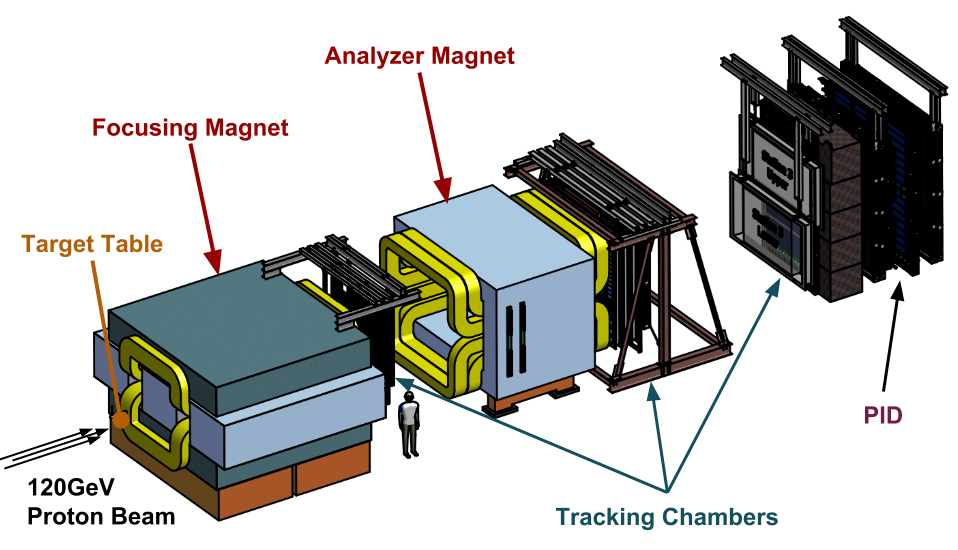
\includegraphics[width=0.75\textwidth]{figures/apparatus/Spectrometer.png}
		\caption{Perspective view of the SeaQuest spectrometer apparatus.}
		\label{fig:spectrometer-perspective}
	\end{center}
\end{figure}

The SeaQuest Spectrometer (Fig. \ref{fig:spectrometer-perspective}) consists of the aforementioned focusing magnet, several tracking chambers that record the positions of charged particles through the length of the spectrometer, and an analyzer magnet to bend the particles between tracking stations. The spectrometer measures particle momenta by recording the bend of each charged particle as it passed through the analyzer magnet, where the magnetic field is known. This is performed by reconstructing the trajectory of a particle in one-half of the spectrometer (before the analyzer magnet) and then similarly reconstructing the trajectory of particles in the other half. If two trajectories can be matched up, then the particle momentum can be extracted by taking the ratio of the magnet's $p_T$-kick to the change in the track's direction.

The spectrometer's geometric design and event triggering selection is optimized to detect oppositely-charged pairs of muons while minimizing the sensitivity to various sources of unwanted backgrounds. Positive identification of muons is achieved by requiring signals in the hodoscopes for known muon \emph{``roads''} along with requiring signals in the proportional tubes located at the farthest end of the experiment, past an iron wall. Electrons and any hadrons are stopped by the solid iron focusing magnet an iron wall farther down while muons will pass through them unencumbered.

The coordinate system is defined as the following: the \emph{z}-axis points along the beam direction, the \emph{y}-axis points upwards vertically, and the \emph{x}-axis lies along the horizontal direction in such a way that a right-handed coordinate system is formed. The terms \emph{upstream} and \emph{downstream} are often used when referring directions or regions in the experimental hall. \emph{Upstream} often refers to the direction towards the beam source ($-z$ direction), while \emph{downstream} refers to the $+z$ direction of the beam trajectory. The origin of the coordinate system was chosen to be the point where the proton beam meets the \emph{upstream}-facing surface of FMAG, the solid focusing magnet.

\section{Main Injector Proton Beam}

\red{Maybe a graphic of FNAL accelerator?}

%% January 7th begin
The Fermilab Main Injector (MI) receives protons that have been accelerated by the Radio Frequency Quadrupoles (RFQ), the Linear Accelerator (LINAC), and the Booster, and it continues to accelerate them from 8 GeV up to the nominal energy of 120 GeV. Along the way, radio-frequency cavity (RFC) accelerators in the LINAC and the MI ``bunches'' up the protons such that the beam has its characteristic 53.1 MHz structure. After the period of acceleration, the protons are then `scraped off' slowly with each passing \emph{turn} of the collected proton beam and sent down the Neutrino-Muon (NM) beam delivery line for approximately five seconds of every minute, called a ``slow spill'' or just ``spill''. Beam is extracted using a resonant process, and the extracted beam retains the 53.1 MHz structure of the Main Injector RFC. Each bunch, or ``bucket'', of protons is less than 2 ns long and the time between bunches is approximately 18.8ns. The spill structure of the beam is depicted in greater detail in Figure \ref{fig:SpillStructure}.

\begin{figure}
	\begin{center}
		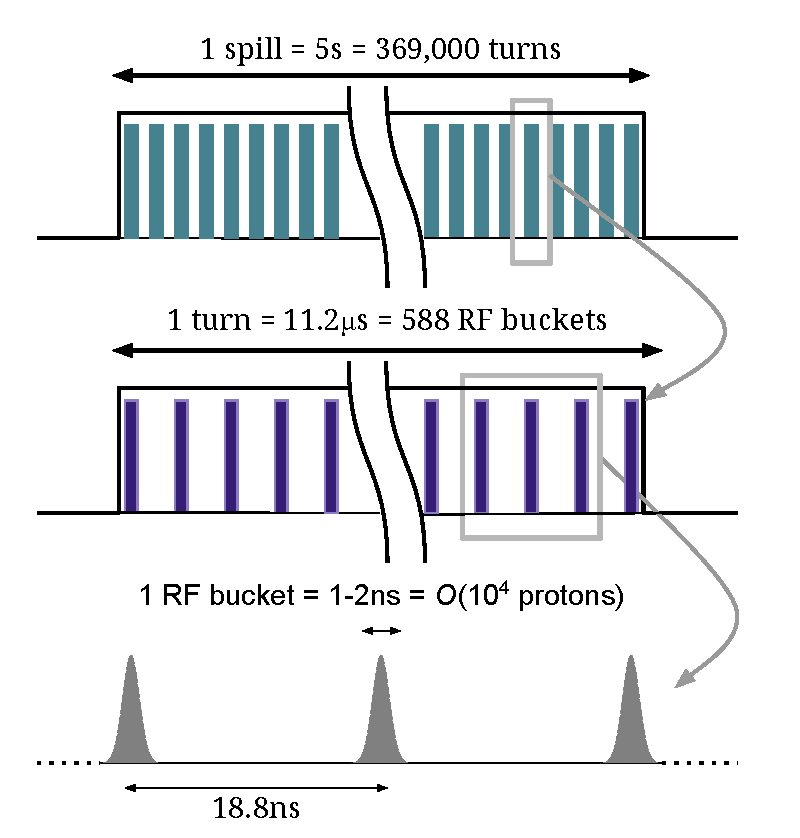
\includegraphics[width=0.55\textwidth]{figures/apparatus/SpillStructure.pdf}
		\caption{Spill structure of the beam delivered to SeaQuest.}
		\label{fig:SpillStructure}
	\end{center}
\end{figure}

The beam sent to SeaQuest is not uniform in time throughout the spill.  There are beam bunches in the MI that are intentionally left empty so that the abort kickers can ramp to a full field during a gap in the beam. There are also bunches left empty to allow the injection kickers to inject 8 GeV protons from the Booster without disturbing bunches of protons already in the Main Injector.  Typically, 498 of the 588 ``RF buckets'' in the Main Injector contain protons during the SeaQuest slow spill cycle.  It is the case, however, for SeaQuest, that the intensity of the bunches corresponding to these 498 full buckets varies greatly throughout the slow spill. On \emph{average}, each bucket will have \emph{$\bigoh$}($10^4$) protons and the spill has an intensity of approximately $2\times 10^{12}$ protons per second and therefore about $1\times 10^{13}$ protons delivered per spill.

Several guiding and focusing magnets bend and deliver beam to the NM beamline which serves both the test beam facility and SeaQuest at NM4. The beam is focused to a width of 250$\mu$m. The profile, position, and intensity are measured along the NM beamline by several detectors. The intensity of the beam is monitored by an ion chamber (IC) and a secondary emission monitor (SEM) in the NM3 sector of the beamline. The beam profile and position are monitored by SWICs and beam-position monitors (BPMs), respectively. The Accelerator Control Network (ACNET) display of the SWIC readout can be seen in Figure \ref{fig:Profile}. The closest BPMs and SWICs to the spectrometer were located in NM2 enclosure. The beam profile does not maintain its 250$\mu$m shape and spreads slightly as it moves towards the spectrometer. The final beam profile is measured by inspecting the upstream-facing side of the solid targets, and it was found to be approximately 6mm wide by 1mm high.

\begin{figure}
	\begin{center}
		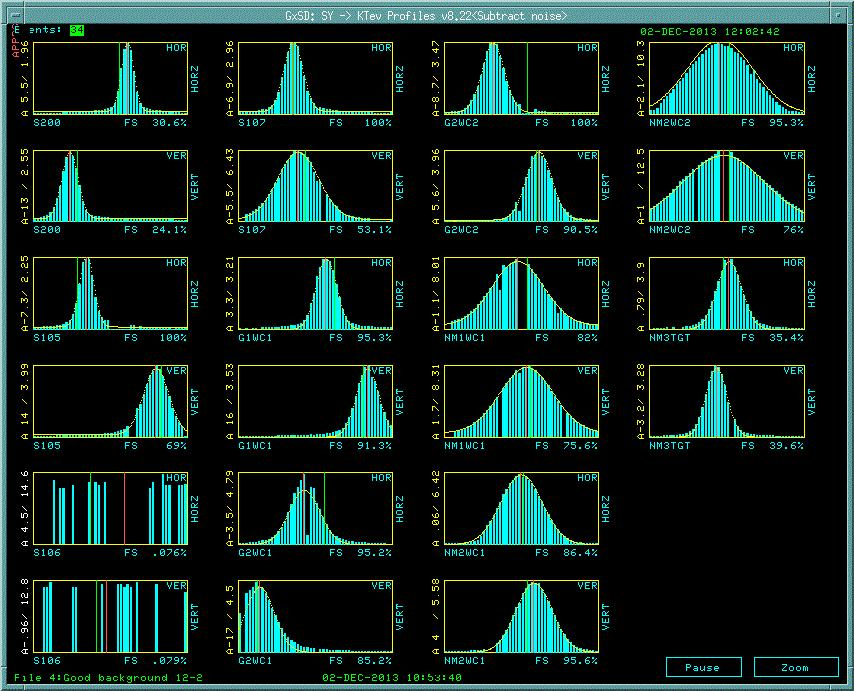
\includegraphics[width=0.65\textwidth]{figures/apparatus/swic.jpg}
		\caption{Beam profile detailed by SWIC detectors along the NM beam line.}
		\label{fig:Profile}
	\end{center}
\end{figure}

\section{Beam Intensity Monitor}

SeaQuest's trigger system (described in detail later) mostly fires on fake dimuons caused by two low $p_T$ muons from unrelated pion decays. The hits in downstream hodoscopes from the pions combined with hits in the upstream hodoscope from two other unrelated particles frequently add up to a false dimuon signal. Since this type of fake trigger involves four unrelated particles, the probability that a trigger will occur increases with $I^4$, where $I$ is the intensity of the beam bucket; the number of protons in the triggered beam bunch.

The SeaQuest data acquisition system (also described later in detail) can read out approximately 3000 events per second without significant dead time.  During the commissioning run of SeaQuest, the trigger rate was very high and the trigger dead time was close to 100\%.  These triggers were taken at such high beam intensities that the occupancy of all SeaQuest detector elements was more than 50$\%$, making pattern recognition essentially impossible (see Figure. \ref{fig:splat}). The Beam Intensity Monitor (BIM) was designed to solve this problem.

\begin{figure}
	\begin{center}
		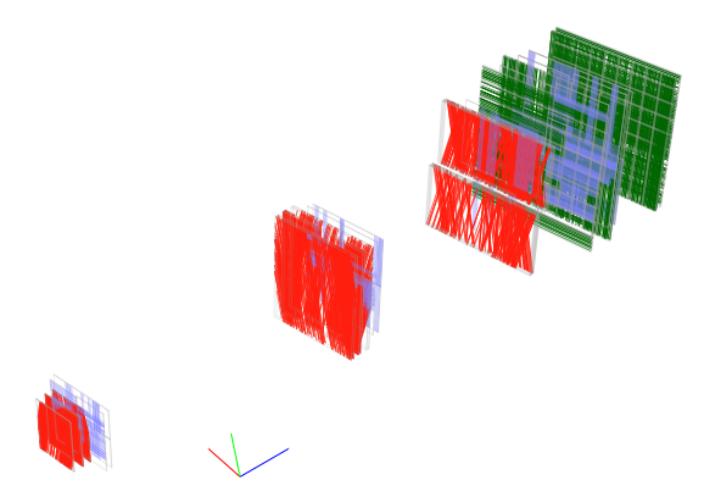
\includegraphics[width=0.5\textwidth]{figures/apparatus/splat2.png}
		\caption{A single high-intensity event with majority of all detector elements firing off. White space within the rectangles indicates inactive elements whereas red, blue, and green represent elements which have fired during that event. Track reconstruction in these cases is impossible.}
		\label{fig:splat}
	\end{center}
\end{figure}

The SeaQuest Beam Intensity Monitor (BIM) senses when the beam intensity is above a programmable threshold. If an RF bucket with an intensity above this threshold is detected, the BIM sends a signal to inhibit certain triggers until the intensity once more falls below the threshold. The inhibit threshold is tuned frequently as trigger and beam conditions change, but it is typically set at $\sim95,000$ protons per RF bunch. For reference, a full RF bucket at an intensity of $2\times 10^{12}$ protons per spill is $\approx$10,000 protons.

The beam intensity is measured using an atmospheric pressure gas \v{C}erenkov counter. A gas mixture of 80$\%$ Argon and 20$\%$ CO$_2$ is used as the \v{C}erenkov radiator. The counter and readout electronics were designed to have $O(ns)$ time resolution, and a linear response over a large dynamic range.  A diagram of the counter is shown in Figure~\ref{fig:BIMCerenkov}.  A 45 degree aluminized Kapton mirror directs light to a single photomultiplier tube.  A \emph{baffle} of black construction paper held parallel to the mirror ensures that the proton path length through the light-radiating gas with respect to the mirror is independent of beam position. A two-inch diameter 8-stage photomultiplier tube (PMT) is positioned close to the mirror so that all \v{C}erenkov light created between the baffle and the mirror falls directly on the aperture of the PMT. It was observed during the commissioning run that after exposure to $\approx 3 \times 10^{17}$ protons (~3 weeks of uninterrupted usage), the mirror reflectivity is significantly reduced in the beam spot, and the mirror then needs to be replaced.

\begin{figure}
	\begin{center}
		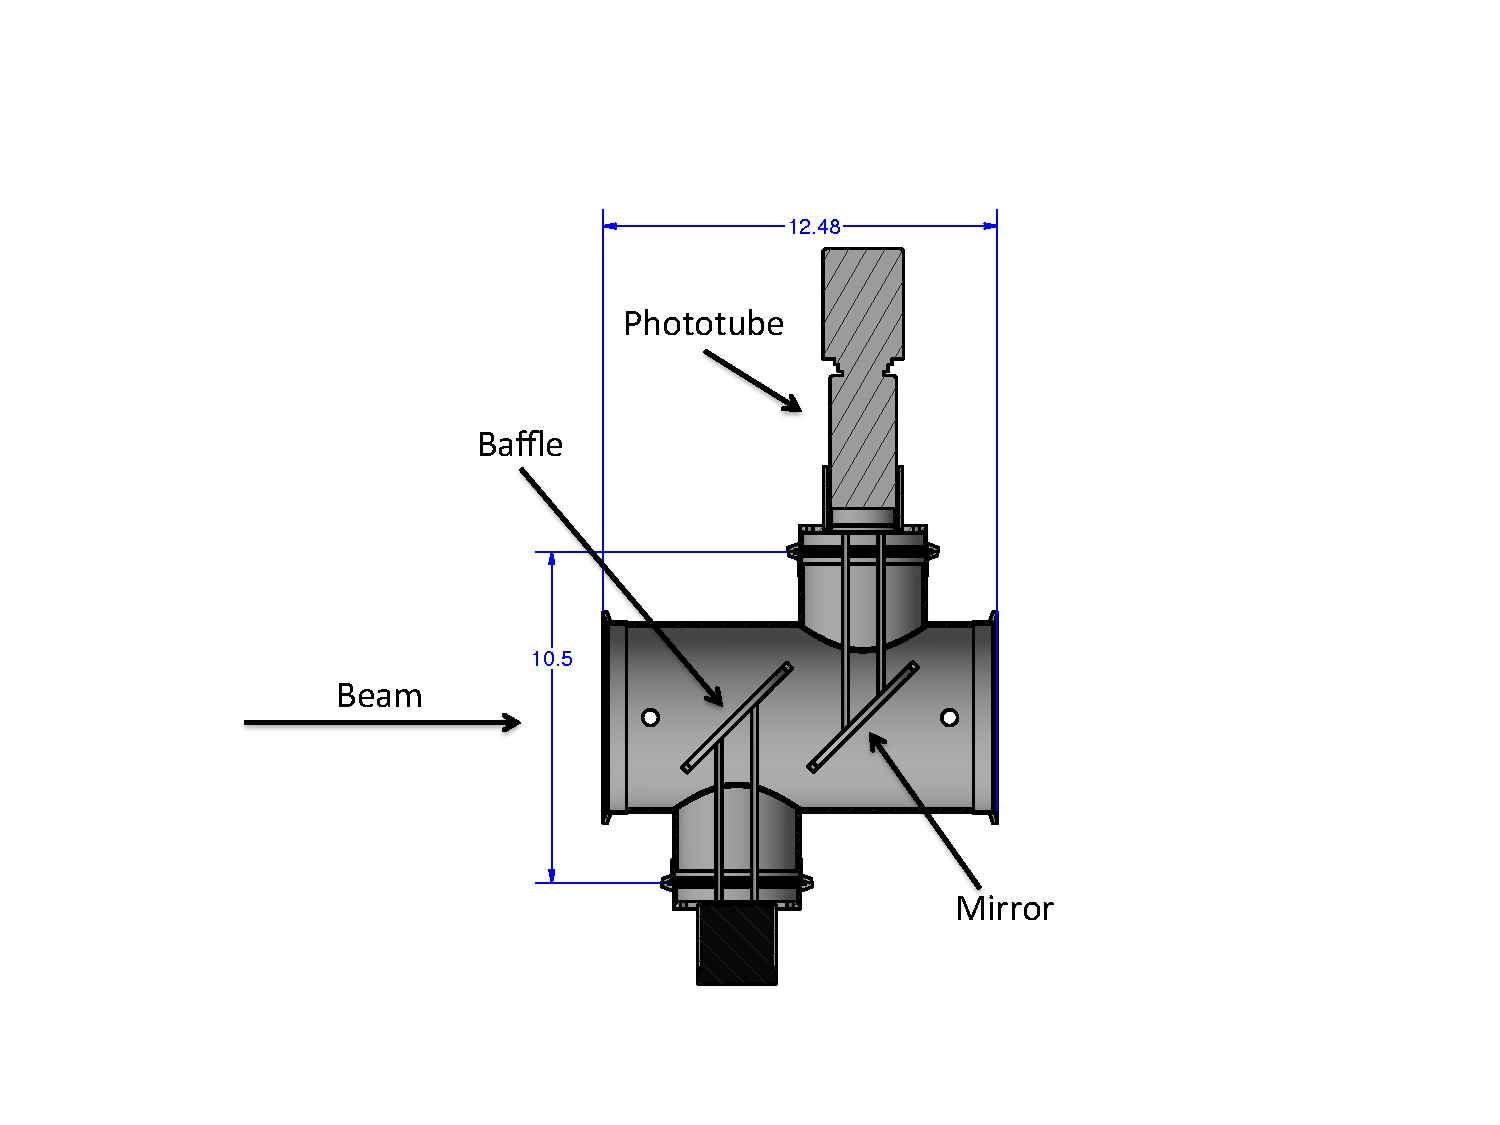
\includegraphics[width=0.6\textwidth]{figures/apparatus/BIMCerenkov.pdf}
		\caption{The Beam Intensity Monitor (BIM) \v{C}erenkov counter. Measurements are in inches.}
		\label{fig:BIMCerenkov}
	\end{center}
\end{figure}

The signal from the BIM is integrated and digitized using a custom charge (Q) integrator and encoder (\emph{QIE}) integrated circuit board, which comes from a family of circuits used first by the KTeV experiment at Fermilab\cite{QIE}. The chip is clocked with the Main Injector RF clock and provides an ADC (analog-digital conversion) every 18.8ns clock cycle. The light incident on the photomultiplier tube is attenuated using neutral density filters (NDF's) so that the QIE least count corresponds to $\sim$30 protons per beam bunch.

In addition to inhibiting triggers during high-intensity periods of beam, the BIM readout module also provides critical information used to calculate the number of protons incident on the SeaQuest targets while the experiment is ready and able to trigger. This value is needed to normalize SeaQuest cross section measurements. The BIM readout module provides the following:
\begin{itemize}
	\item Sum of all ADC signals for the entire spill (QIESum).
	\item Sum while inhibit is asserted at trigger logic.
	\item Sum during trigger dead time.
	\item A snapshot of beam intensity 16 buckets before and after the triggered RF bucket
\end{itemize}

These are used to calculate a ratio of protons that were `live' (the experiment can trigger) via the following:
\begin{eqnarray}
\%live & = & \frac{QIESum - (inhibit\ sum + dead\ time\ sum)}{QIESum} \\
liveProton & = & totalProton \cdot \%live
\label{eqn:liveproton}
\end{eqnarray}
where ``totalProton'' is the intensity value recorded from the SEM detector located just upstream of the BIM \v{C}erenkov counter. The SEM itself is calibrated by foil activation. The snapshot of the triggered RF bucket intensity along with the 32 surrounding RF bucket intensities is used for studies and corrections of the rate-dependent effects on detector efficiencies and reconstructed measurements.

\section{The SeaQuest Targets}

\begin{table}[p]
	\begin{center}
		\begin{tabular}{c c c c c c c}
			\parbox{1.5cm}{\centering{~\\Position} } & \parbox{1.5cm}{\centering{~\\Material} }  &\parbox{1.5cm}{\centering{Density\\{[g/cm$^3$]}} }  &  \parbox{1.75cm}{\centering{Thickness\\{[cm]}} }& \parbox{2cm}{\centering{Interaction\\Length} }&  \parbox{1.5cm}{\centering{Spills/\\Cycle\\(\%spills)} } \\ [0.5ex] \hline
			1 & $H_2$     & 0.07065 & 50.8  & 0.06902 & 10 (43\%) & \\
			2 & Empty     & NA      & NA    & 0.0016  & 2 (9\%)  & \\
			3 & $D_2$     & 0.1617  & 50.8  & 0.1144  & 5 (22\%)  & \\
			4 & None      & NA      & NA    & 0.0     & 2 (9\%)  & \\
			5 & Iron      & 7.874   & 1.905 & 0.1135  & 1 (4\%)  & \\
			6 & Carbon    & 1.802   & 3.322 & 0.0697  & 2 (9\%)  & \\
			7 & Tungsten  & 19.30   & 0.953 & 0.0958  & 1 (4\%)  & \\ [0.5ex] \hline
		\end{tabular}
		\caption{Characteristics of the seven SeaQuest target positions.  The ``Spills/Cycle'' is only a typical configuration and can vary according to needs and running configurations.  The non-zero interaction length of the empty flask is due to the 51$\mu$m-thick stainless steel end-caps of the flask and the 140 $\mu$m-thick titanium windows of the vacuum vessel that contains it.}
		\label{tab:target-materials}
		
	\end{center}
\end{table}

\begin{figure}[p]
	\begin{center}
		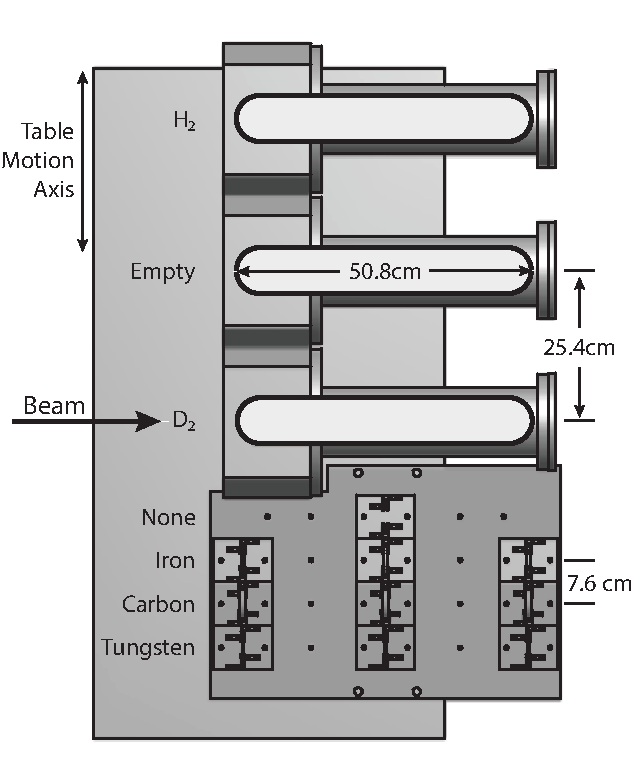
\includegraphics[width=0.65\textwidth]{figures/apparatus/target-tableLayout.pdf}
		\caption{The layout of the target table and its seven target positions, as seen from above.}
		\label{fig:table-layout}
	\end{center}
\end{figure}


A wide range of atomic weights (from 2 to 184) is required to do an A-dependence study of the Drell-Yan process. At SeaQuest, the targets used are $^1H (\ell),\ ^2H (\ell),\ C,\ Fe,\ $and$\ W$. In addition to the two liquid targets and the three solid targets, two positions on the target table were used for measuring background signal rates: an empty flask, identical to the flasks used for the $^1H$ and $^2H$ targets, and a single empty solid target holder. Colloquially speaking: the $^1H$ target is interchangeably referred to as the liquid hydrogen target, $\ell H_2$, \emph{LH2}, or $H_2$; $^2H$ is likewise referred to as the liquid deuterium target, $\ell D_2$, \emph{LD2}, or $D_2$; the empty flask is referred to as the ``Empty'' target; the empty solid target holder is referred to as the ``None'' target.

These are all mounted on a laterally-moving, remotely positionable table (in the $\pm x$ direction), able to move over a range of 91.4cm. The table's center is located at $(0, 0, -1.25)$ meters, directly in front of the upstream face of FMAG, the solid iron focusing magnet. Because of the $\sim$5.0cm diameter of the targets and the 6x1mm dimensions of the beam, the targeting efficiency was 100\%. The details of the target materials are summarized in Table \ref{tab:target-materials}, and the layout of the target table can be seen in \ref{fig:table-layout}.

The $H_2$ gas used is ``Ultra High Purity 5.0 Grade'' or 99.999\% pure.  The deuterium has come from two different sources.  The first of these is a Fermilab-provided supply of gas left over from previous bubble chamber experiments. This gas was known to have a small hydrogen contamination and was measured by mass spectroscopy to have a composition of 85.2\% D$_2$, 12.7\% HD, 1.2\% $^4$He, and 0.8\% H$_2$ by mole. As the analysis of experimental data commenced, handling the ramifications of the D$_2$ impurity came under focus. Unexpected bottle-to-bottle variation in contamination became evident, and the sample-taking methodology itself for spectroscopy became suspect of introducing contamination. In order to no simplify analysis and reduce the substantial complexity and cost of further gas analysis, SeaQuest switched to commercially available ``Research Grade'' D$_2$, which is better than 99.6\% pure with virtually all HD to balance. The data analyzed in this paper deals with the impure D$_2$ target material before this switch. Further information on the D$_2$ composition and how it is handled in the context of analysis will be covered in Chapter 5.

%10'' apart to approximate the 20'' 
%  more closely spaced (6.73'').
Each of the three solid target positions is divided into three disks of 1/3 the total thickness provided in Table \ref{tab:target-materials}. These disks are spaced 25.4cm apart to approximate the distribution of the liquid target, thereby minimizing target-dependent variation in spectrometer acceptance. The one exception to this is that during the Run II period the iron disks were more closely spaced (17.1cm). The decision to place these iron disks closer together than the rest during Run II is still unclear.

The target table is able to move between two different targets in about 30 seconds. This allows a change between targets in the 55 seconds between successive spills. With this frequent target interchange, the systematic uncertainties associated with drifts in beam characteristics, monitor gains, and detector efficiencies are reduced to a minimum when investigating A-dependent ratios. How much beam time each target received is determined by interaction lengths of the targets along with the amount of statistics desired for certain targets. As the flagship measurement of SeaQuest is the $\bar{d}/\bar{u}$ asymmetry, more emphasis was placed on the hydrogen and deuterium than the nuclear targets. The spills per cycle and beam time allocation can be found in Table \ref{tab:target-materials}.

\section{Focusing and Analyzing Magnets}

Two large dipole magnets are used in the experiment to be select forward going ($x_F > 0$) dimuons, reject low-momentum particles, and analyze their kinematic characteristics. The most upstream magnet, denoted ``FMAG'', is a solid iron A-frame magnet with an aperture of 1.22m in the $x$-direction and 66cm in the $y$-direction. It is assembled from 43.2cm x 160cm x 503cm iron slabs, as shown in Fig.~\ref{fig:FMag}. The magnet has no air gap, and the iron has extremely high purity, allowing a 2000A excitation current to generate a nearly constant, central magnetic field of 1.9 Tesla (yielding a 2.91 GeV/c total magnetic deflection). The field is generated by exciting the embedded aluminum \emph{``bedstead''} coil to 2000 Amps at 25 Volts (50 kW).  The current exciting FMAG is monitored by the Fermilab ACNET system and is broadcast to the SeaQuest slow data acquisition system every acceleration cycle. The excitation is also input to the beam-disabling safety system in order to prevent the beam from hitting the SeaQuest spectrometer when FMAG is not fully powered. FMAG also acts as the beam dump for the 120 GeV beam. There is a 5cm diameter by 25cm deep bore drilled into the upstream end of FMAG (recall, this is the origin of the experiment's coordinate system).  The 120 GeV protons that do not interact in the SeaQuest targets 125cm upstream of FMag, interact in the central iron slab.  Most of the 2.0 kW beam power is dissipated in this slab and is eventually conducted to the coils and external surfaces to be radiated away.

\begin{figure}
	\centering
	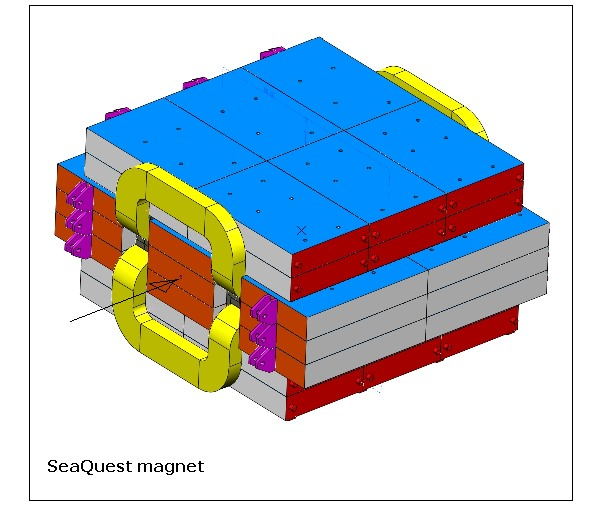
\includegraphics[width=8cm]{figures/apparatus/FMAG}
	\caption{Perspective drawing of FMAG's aluminum coils embedded in an arrangement of iron slabs.}
	\label{fig:FMag}
\end{figure}

The downstream magnet, denoted ``KMAG'', is a 300cm long iron rectangular magnet with a 289cm wide by 203cm high central air gap.  It was originally constructed by the KTeV collaboration\cite{PhysRevD.67.012005} at Fermilab.  It is excited to a central field of 0.4 Tesla (0.402 GeV/c magnetic deflection) by 1600 Amps at 270 Volts (430kW).  The spatial distribution of the magnetic field in KMAG was measured by the KTeV group and re-verified by SeaQuest.  In normal running conditions, both FMag and KMAG bend muons horizontally in the same direction. This two-magnet configuration is often referred to as a focusing spectrometer.

The 2.91 GeV/c and 0.402 GeV/c magnetic deflections deliver a transverse-momentum ($p_T$) kick along the to charged particles passing through the spectrometer. The magnets bend the paths of the muon in the $\pm x$ direction, with the sign depending on the orientation of the magnetic fields and the particles' charges. Between Run II and Run III of data taking, the current direction was reversed, thereby reversing the direction of the magnetic fields. During Run II, the magnetic fields were pointing in the $-y$ direction, and in Run III, the magnetic fields were flipped to point in the $+y$ direction. This was done for two reasons: (1) to identify any left-right asymmetries in the experiment, and (2) to limit the amount of radiation on the electronics in the experimental hall, as a large number of positive particles were being swept directly towards the electronics racks during Run II.

\red{Note: Maybe add something track resolution effects due to multiple scattering in FMAG? Or save for Analysis chapter?}

\section{Beam Dump, Shields, and Absorbers}

In order to prevent damage to the downstream detectors from the beam and reduce signals from incidental radiation, the spectrometer is designed with a beam dump and two hadron absorber walls. Approximately 125cm downstream of the target table is the water-cooled beam dump whose upstream face is located at $(0.0, 0.0, 0.0)$ m. The beam dump is one of the many solid iron 5m blocks that fill and surround the FMAG coils. The whole length of the beam dump along the beam axis is equivalent to $\approx 35$ nuclear interaction lengths of iron. 

Between the downstream face of FMAG and Station 1, there is a 2 cm thick wall of borated polyethylene which is put in place as a fast neutron shield. This material is 5\% boron by weight, with the rest being polyethylene. The polyethylene contains high hydrogen content, making it an effective fast neutron radiation shield, slowing down the fast neutrons down to thermal speeds. The boron in the material provides attenuation of thermal neutrons, thus reducing the levels of capture-gamma radiation elsewhere in the experiment. Borated polyethylene at this thickness is a common and optimal neutron shielding material for areas of low to intermediate neutron flux where the temperature is below $82^\circ$C \CN. These conditions make the downstream side of FMAG ideal for its placement.

Farther downstream, there is another hadron absorber wall located between Station 3 and Station 4. The absorber wall consists of a stack of 98cm thick iron blocks. This is an equivalent of $\approx 6$ nuclear interaction lengths. The purpose of this wall is to identify muons at the rear of the apparatus by effectively blocking all other types of particles. The only charged particles which can penetrate this absorber wall that weren't swept away by either magnet are muons.

\section{Tracking Detectors}

The tracking detectors are the instruments used for measuring the values of the kinematic variables of the dimuon pairs. Several different types of detectors are grouped together to form a detector \emph{Station}. The types of detectors used are hodoscopes, wire chambers, and proportional tubes. There are four stations throughout the experimental hall that provide tracking information at different points along the spectrometer, numbered from 1 to 4 in order of increasing $z$. Station 1 is located between FMAG and KMAG. Station 2 is located at the downstream face of KMAG. Station 3 and 4 are just upstream and downstream, respectively, of the iron absorber wall. The Station layout can be seen in Fig. \ref{fig:stations}

\begin{figure}
	\centering
	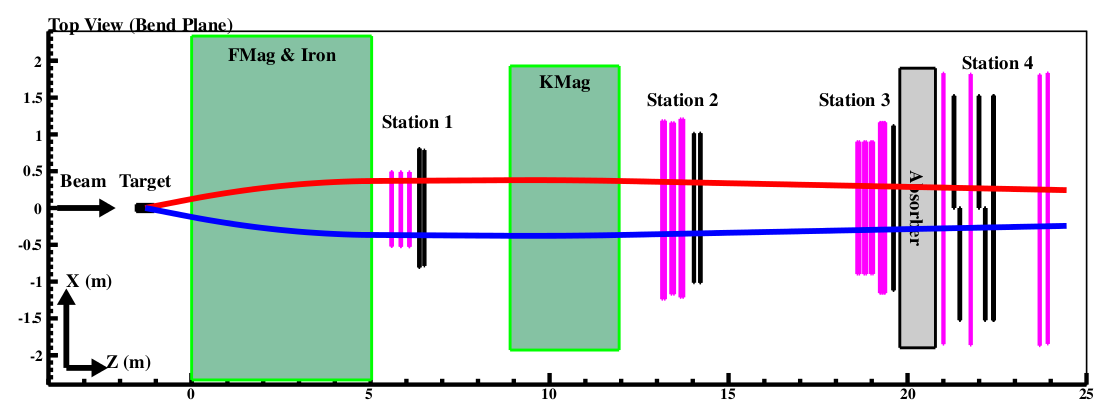
\includegraphics[width=0.75\textwidth]{figures/apparatus/stations.png}
	\caption{Spectrometer layout of FMAG, KMAG, and Detector Stations 1-4.}
	\label{fig:stations}
\end{figure}

\subsection{Triggering Hodoscopes}

Hodoscope arrays are located at each of the four detector stations. These detectors' primary usage is to select events with two opposite-signed muon tracks in them. Certain `roads' through the spectrometer are defined in the fast trigger logic, and when two desired roads are observed in a given event, the trigger system tells the data acquisition systems to record that event's data. In addition to this, the hodoscopes provide analysts with the ability to discard or ignore certain hits in adjacent chambers for which there is no corresponding nearby hodoscope hit. This is useful in decreasing the hit multiplicities in the wire chambers, which in turn decreases the combinatoric complexity of reconstruction algorithms.

Each of the eight hodoscope planes is split into two halves: top and bottom in the case of planes with vertically-oriented paddles, or left and right for planes with horizontally-oriented paddles (denoted by `T', `B', `L', and `R', respectively). In each half-plane, the hodoscopes are a set of long rectangles arranged `picket fence'-style with a small 0.3175cm overlap, as to prevent any particles from possibly slipping between paddles. A single hodoscope detector element is composed of plastic scintillator material connected to Philips XP 2008 photomultiplier tubes (PMT) by plexiglass light guides. Stations 1, 2, and 4 each have two hodoscope planes, with planes of both vertically- and horizontally-oriented paddles (for measuring in $x$ and $y$, respectively). Station 3 consists only of vertically-oriented plane, and thus measures in the $x-$direction only, which is in the experiment's $x-z$ bend plane. The hodoscope planes are named according to detector station and the direction that they measure. For example, the $y$-measuring hodoscope plane in Station 2 is called ``H2Y''. The individual half-planes are named according to detector station and which half it is of the two. For example, the top half of the $x$-measuring hodoscope plane in Station 1 is referred to as ``H1T''. As such, the ``H3X'' detector is composed of ``H3T'' and ``H3B''. The detailed specifications of each hodoscope plane are given in Table \ref{tab:hodoscopes}. A precise alignment of the hodoscopes was achieved by examining the distributions of positions of tracked muons at each hodoscope plane when a given hodoscope element in that plane was fired.

\begin{table}[bthp]\centering
	\begin{tabular}{llllll}
		\hline
		\hline
		Detector & Paddle & Overlap & \# of paddles & Width $\times$ Height & $z$-position [cm] \\
		& Width & [cm] & (per half-plane) & (per half-plane) &  \\
		& [cm] & & & [cm] $\times$ [cm] & \\
		\hline
		H1X & 7.32 & 0.3175 & 23 & 162 $\times$ 70 & 666 \\
		H1Y & 7.32 & 0.3175 & 20 & 79 $\times$ 140 & 653 \\
		H2X & 13.00 & 0.3175 & 16 & 203 $\times$ 152 & 1421 \\
		H2Y & 13.00 & 0.3175 & 19  & 132 $\times$ 241 & 1400 (L), 1406 (R) \\
		H3X & 14.59 & 0.3175 & 16  & 228 $\times$ 168 & 1959 \\
		H4X & 19.65 & 0.3175 & 16  &  305 $\times$ 183 & 2234 (T), 2251 (B) \\
		H4Y1 & 23.48 & 0.3175 & 16  & 152 $\times$ 366 & 2130 (L), 2146 (R) \\
		H4Y2 & 23.48 & 0.3175 & 16  & 152 $\times$ 366 & 2200 (L), 2217 (R)\\
		\hline
		\hline
	\end{tabular}
	\caption{Parameters of all hodoscope planes. $z$-positions of H2Y and H4 half-planes are offset slightly due to the half-planes themselves overlapping.}
	\label{tab:hodoscopes}
\end{table}

\subsection{Drift Chambers}

Each of Stations 1, 2 and 3 is equipped with a drift chamber (DC) to measure the passing $x$ and $y$ positions of muons at its $z$ location, with each DC flat vertical to the $z$ axis, and a drift cell is of the box shape. These measured positions are critical for reconstructing the trajectory of muons, and thereby their kinematics. Each DC contains six drift chamber planes, arranged in three pairs with parallel wire orientations (each pair referred to as a ``view''). Wires oriented vertically ($x$-measuring) are referred to as being in the ``X'' view and at angles of $+14^\circ$ and $-14^\circ$ with respect to the $y$-axis are the ``V'' and ``U'' planes, respectively. The second plane in each view is offset from the first by one-half of a wire-to-wire distance (\emph{``cell width''}) in order to resolve the left-right ambiguity of drift direction. This offset plane of each pair is referred to as the \emph{primed} plane, and is denoted with a `$\prime$'. So, in each DC, there are X, X$^\prime$, U, U$^\prime$, V, and V$^\prime$ planes, with primed and unprimed planes (like X and X$^\prime$) constituting a view.

The individual drift chambers at Stations 1 and 2 are called ``D1'' and ``D2'', respectively. Station 3 has two drift chambers since the desired acceptance area it has to cover is substantially larger than one DC can cover. These are split vertically to cover the top and bottom halves, and are called ``D3p'' and ``D3m'' where ``p'' and ``m'' stand for ``plus'' and ``minus''. Table~\ref{table:cham:param} summarizes the parameters of the DC's. D1 and D3m have been upgraded during the data taking, as listed in Tab.~\ref{tab:cham:comb1}. This original and upgraded versions are referred to as D$N$.1 and D$N$.2, respectively.

\begin{table}[bthp]\centering
	\begin{tabular}{cc|cccc}
		\hline \hline
		Chamber & Plane & Number   & Cell  & Width            & $z$-position \\
		&       & of wires & width & $\times$ height  &      \\ 
		&       &          & [cm]  & [cm] $\times$ [cm] & [cm] \\ 
		\hline
		D1.1    & X     & 160      & 0.64  & 102 $\times$ 122 &  617    \\
		& U, V  & 201      & 0.64  & 101 $\times$ 122 & $\pm$20 \\
		D1.2    & X     & 320      & 0.50  & 153 $\times$ 137 &  617    \\
		& U, V  & 384      & 0.50  & 153 $\times$ 137 & $\pm$1.2 \\
		D2      & X     & 112      & 2.1   & 233 $\times$ 264 & 1347    \\
		& U, V  & 128      & 2.0   & 233 $\times$ 264 & $\pm$25 \\
		D3p     & X     & 116      & 2.0   & 232 $\times$ 166 & 1931    \\
		& U, V  & 134      & 2.0   & 268 $\times$ 166 & $\pm$6  \\
		D3m.1   & X     & 176      & 1.0   & 179 $\times$ 168 & 1879    \\
		& U, V  & 208      & 1.0   & 171 $\times$ 163 & $\pm$19 \\
		D3m.2   & X     & 116      & 2.0   & 232 $\times$ 166 & 1895    \\
		& U, V  & 134      & 2.0   & 268 $\times$ 166 & $\pm$6  \\
		\hline
		\hline
	\end{tabular}
	\caption{Parameters of all chambers.
		Those of primed planes are almost the same as of unprimed planes.
		The $z$-positions of U and V planes are relative to those of X planes.
	}
	\label{table:cham:param}
\end{table}

\begin{table}[bthp]\centering
	\begin{tabular}{ccc}
		\hline
		Run & Period & Chamber combination \\
		\hline
		1 & 2012 Mar.-2012 Apr.  &  D1.1, D3m.1 \\
		2 & 2013 Nov.-2014 Aug.  &  D1.1, D3m.2 \\
		3 & 2014 Nov.-2015 May   &  D1.1, D3m.2 \\
		3 & 2015 Jun.-2015 Jul.  &  D1.2, D3m.2 \\
		4 & 2015 Sep.-   &  D1.2, D3m.2 \\
		\hline
	\end{tabular}
	\caption{Combination of D1 and D3m chambers per data taking period.}
	\label{tab:cham:comb1}
\end{table}

The acceptance size of each chamber has been adjusted with a Drell-Yan event simulation in order to be as sensitive as possible to the $x_2$ range of interest. Particularly, the greater the acceptance width is, the higher the reach in $x_2$ is. This makes the hit-rate tolerance of the chambers a key feature because the spectrometer is exposed to a large number of background particles, particularly near the edges where the desired $x_2$ events occur. It is particularly significant for the most-upstream station (i.e.~Station 1) which receives the highest hit rates. Experimental data shows that the rate tolerances are 3.0 MHz/wire at D1, 1.6 MHz/wire at D2 and 0.7 MHz/wire at D3 with a beam intensity of $5\times 10^{12}$ protons/spill. The gas-amplification gain should not be degraded under these hit rates.

For Run 2 and beyond, the gas mixture used for almost all the chambers is Argon:Methane:CF4 (88\%:8\%:4\%) with a drift velocity of about 20 $\mu$m/ns. A ``fast gas'' mixture used for D1.2 (upgraded D1) is Argon:CF4:Isobutane:Methylal (68\%:16\%:13\%:3\%) with a drift velocity of 50 $\mu$m/ns and thereby a better hit-rate tolerance. This is ``fast'' in comparison to the $\approx 20\mu$m/ns rest of the DCs. The spatial resolution of each plane is required to be 400$\mu$m, which corresponds to a momentum resolution of $\Delta p / p = 0.03 \cdot p$ (GeV/$c$). The resolution of dimuon invariant mass is dominated by the multiple scattering in FMAG; the chamber momentum resolution is about 10\% of the total mass resolution at maximum.

The D1.1, D2, and D3m.1 chambers have been inherited from previous Drell-Yan experiments that have been conducted at Fermilab.
Chambers D2 and D3m.1 have their origin in E-906~\cite{PhysRevD.43.2815} and D1.1 is from SeaQuest's direct predecessor, E-866/NuSea~\cite{PhysRevLett.80.3715, Towell:2001nh}. Since these chambers have not been used for decades since E-866, they had to be refurbished by restringing $\approx 30\%$ of their sense wires due to them being loose or broken. Newly supplied electronic readout boards were also mounted on these chambers.

The D3p and D3m.2 chambers were designed and constructed specifically for this experiment in order to cover the large acceptance required at Station 3. D3p was newly constructed by the TokyoTech SeaQuest collaborators and was shipped from Japan to Fermilab. The first part of data taking, Run 1, was carried out using D3m.1 while preparing for the construction of D3m.2. The newer D3m.2 is wider than D3m.1 by 25 cm at each side, allowing the high-$x_2$ statistics on $\bar{d}/\bar{u}$ and $Y_A / Y_{^2H}$ to increase by $\approx 20\%$ at $x_2 \sim 0.3$ and $\approx 10\%$ at $x_2 \sim 0.4$. The operational stability also improved, as D3m.1 suffered from frequent dead/noisy wires, HV trips, and leak currents. The D1.2 chamber was also designed and constructed for this experiment by the University of Colorado Boulder. As it is wider than D1.1 by 25 cm at each side and greater hit-rate tolerance, the anticipated statistics is expected in the high-$x_2$ region is expected to increase still more. It was installed in the experimental hall near the end of Run 3.

\subsection{Proportional Tubes}

Downstream of Station 3 and the 1 m thick iron hadron absorber wall is Station 4 with its hodoscope planes and proportional tube  detectors (prop tubes). At Station 4, the only beam-induced particles that remain that can leave tracks in an ionization detector are high energy muons. The prop tubes enable the task of muon particle identification (PID) for the experiment and consist of four planes. Each detector plane is made of 9 prop-tube modules, with each module assembled from 16 12-ft long 2" diameter prop-tubes staggered to form two sub-layers. The first and fourth planes are oriented along the horizontal direction (tubes parallel to the floor) to provide positional measurements in $y$, as shown in Fig.~\ref{fig:proptube:xzview}. The second and third planes are arranged vertically to measure $x$-position as shown in and Fig.~\ref{fig:proptube:yzview}.

\begin{figure}
	\centering
	\begin{minipage}[t]{0.49\linewidth}
		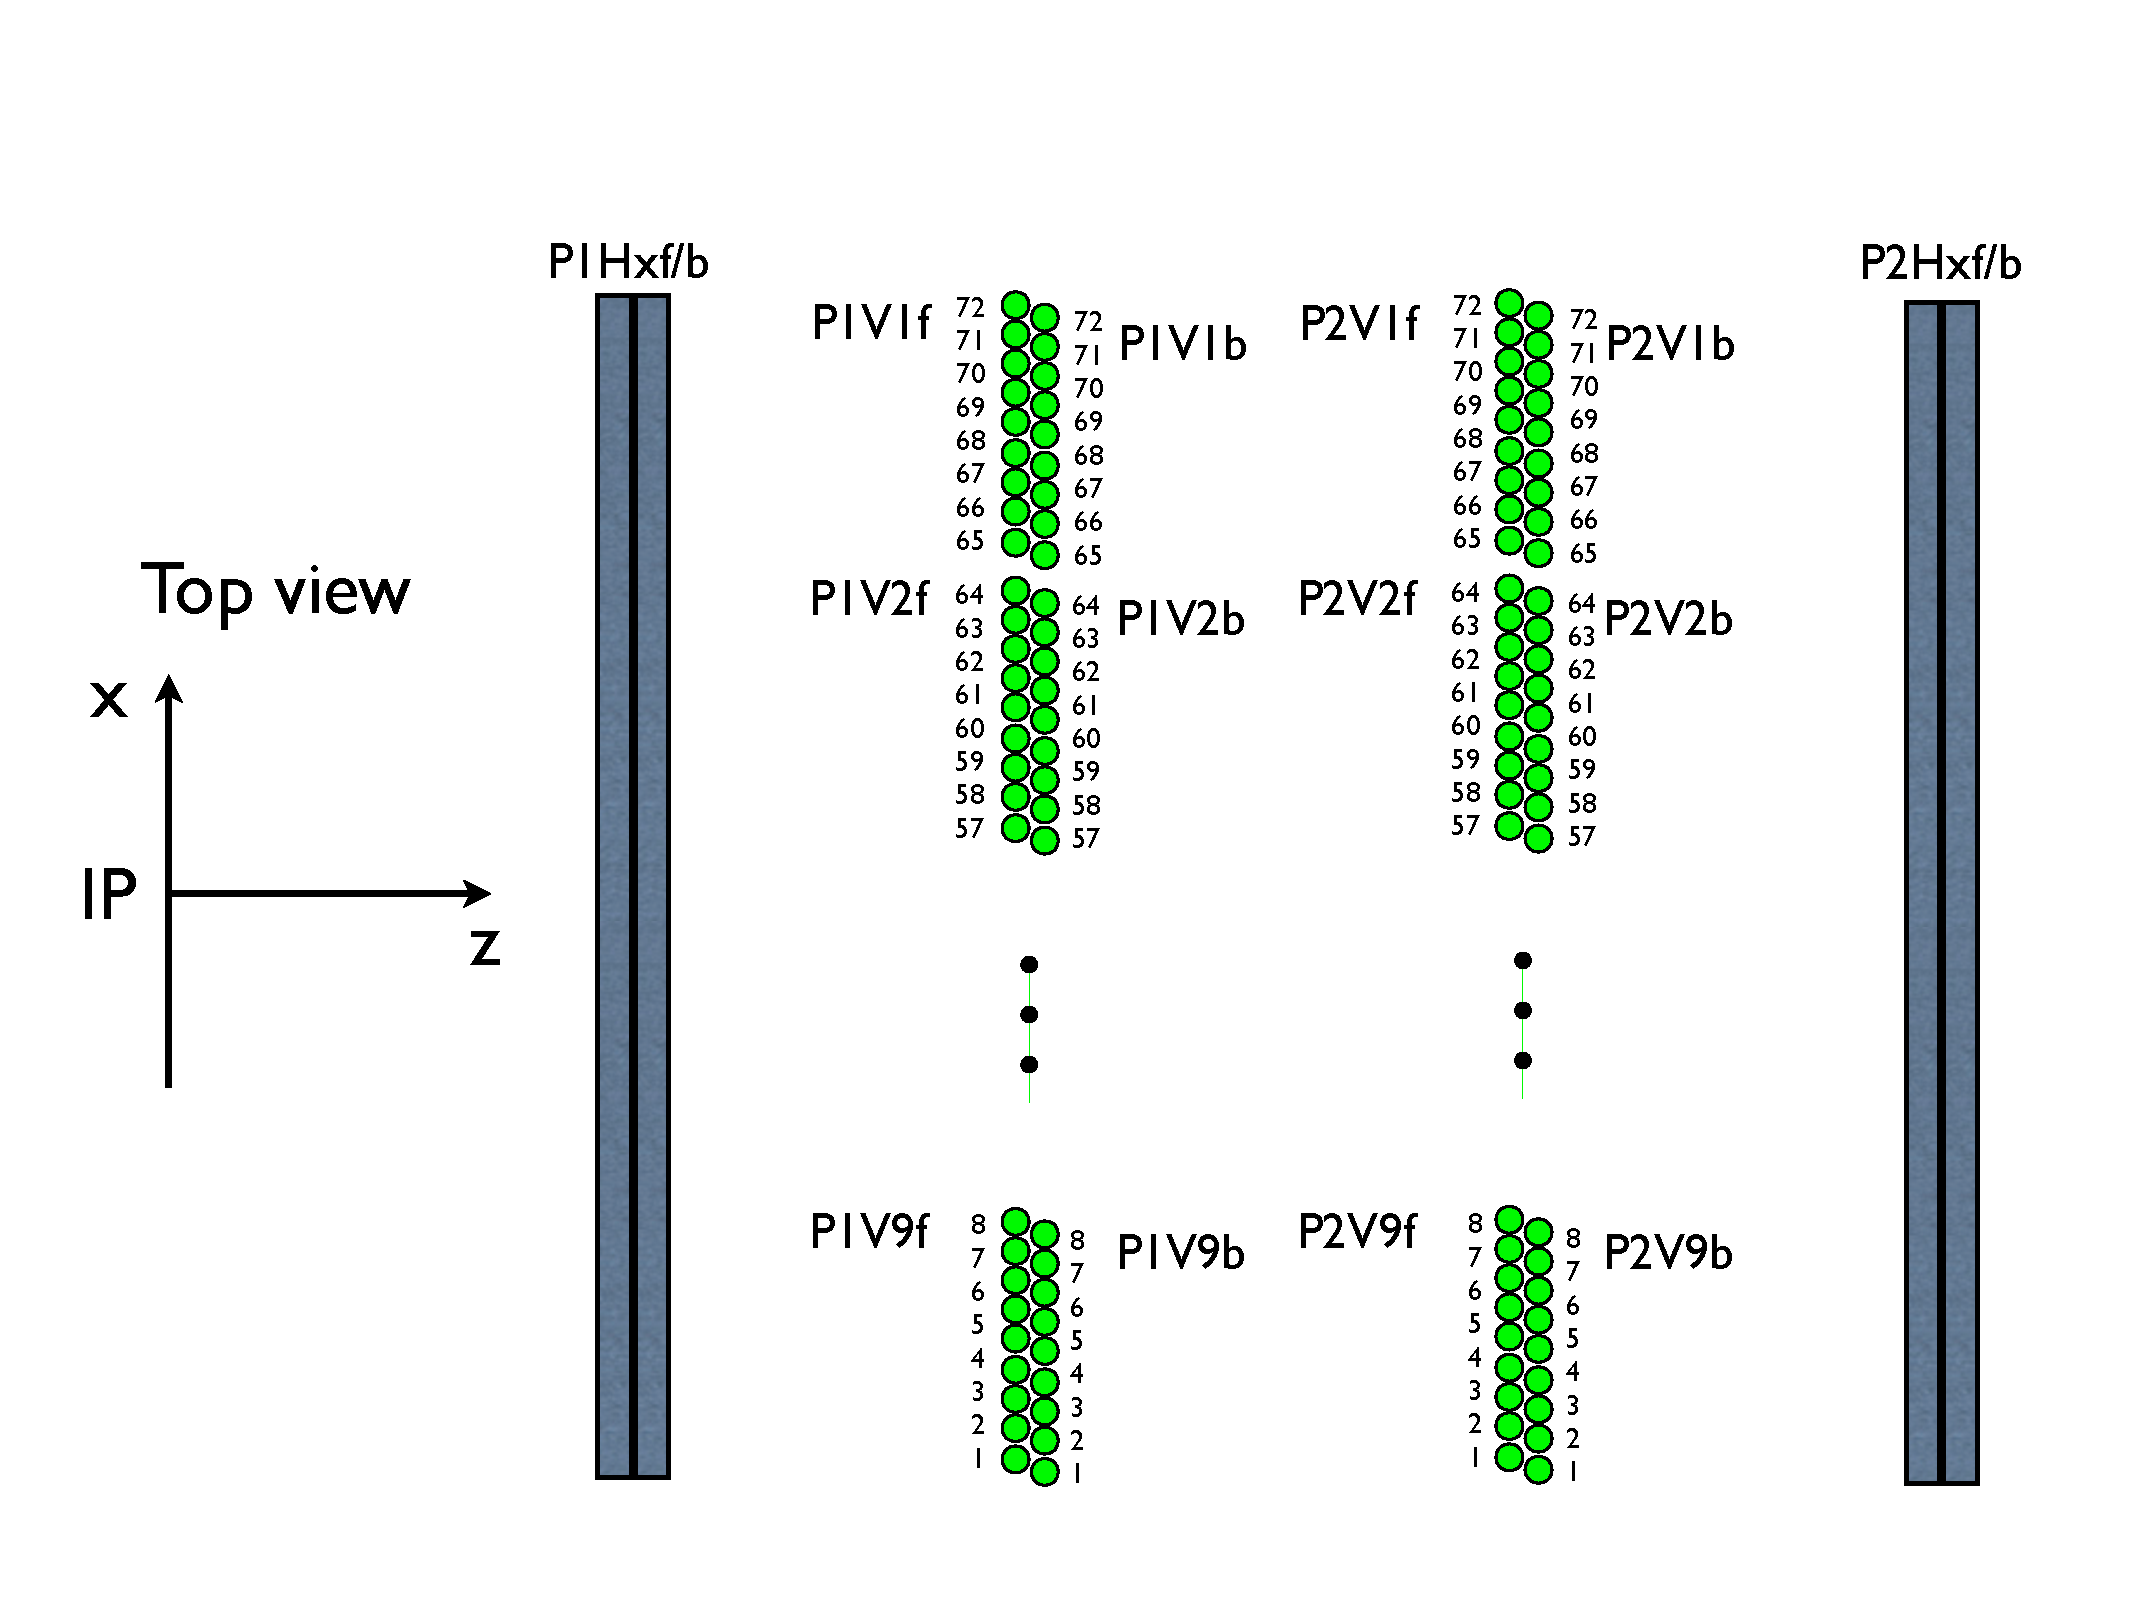
\includegraphics[width=\linewidth]{figures/apparatus/proptubeview_xz.pdf}
		\caption{Proportional tube top ($x-z$ plane) view.}
		\label{fig:proptube:xzview}
	\end{minipage}
	\begin{minipage}[t]{0.49\linewidth}
		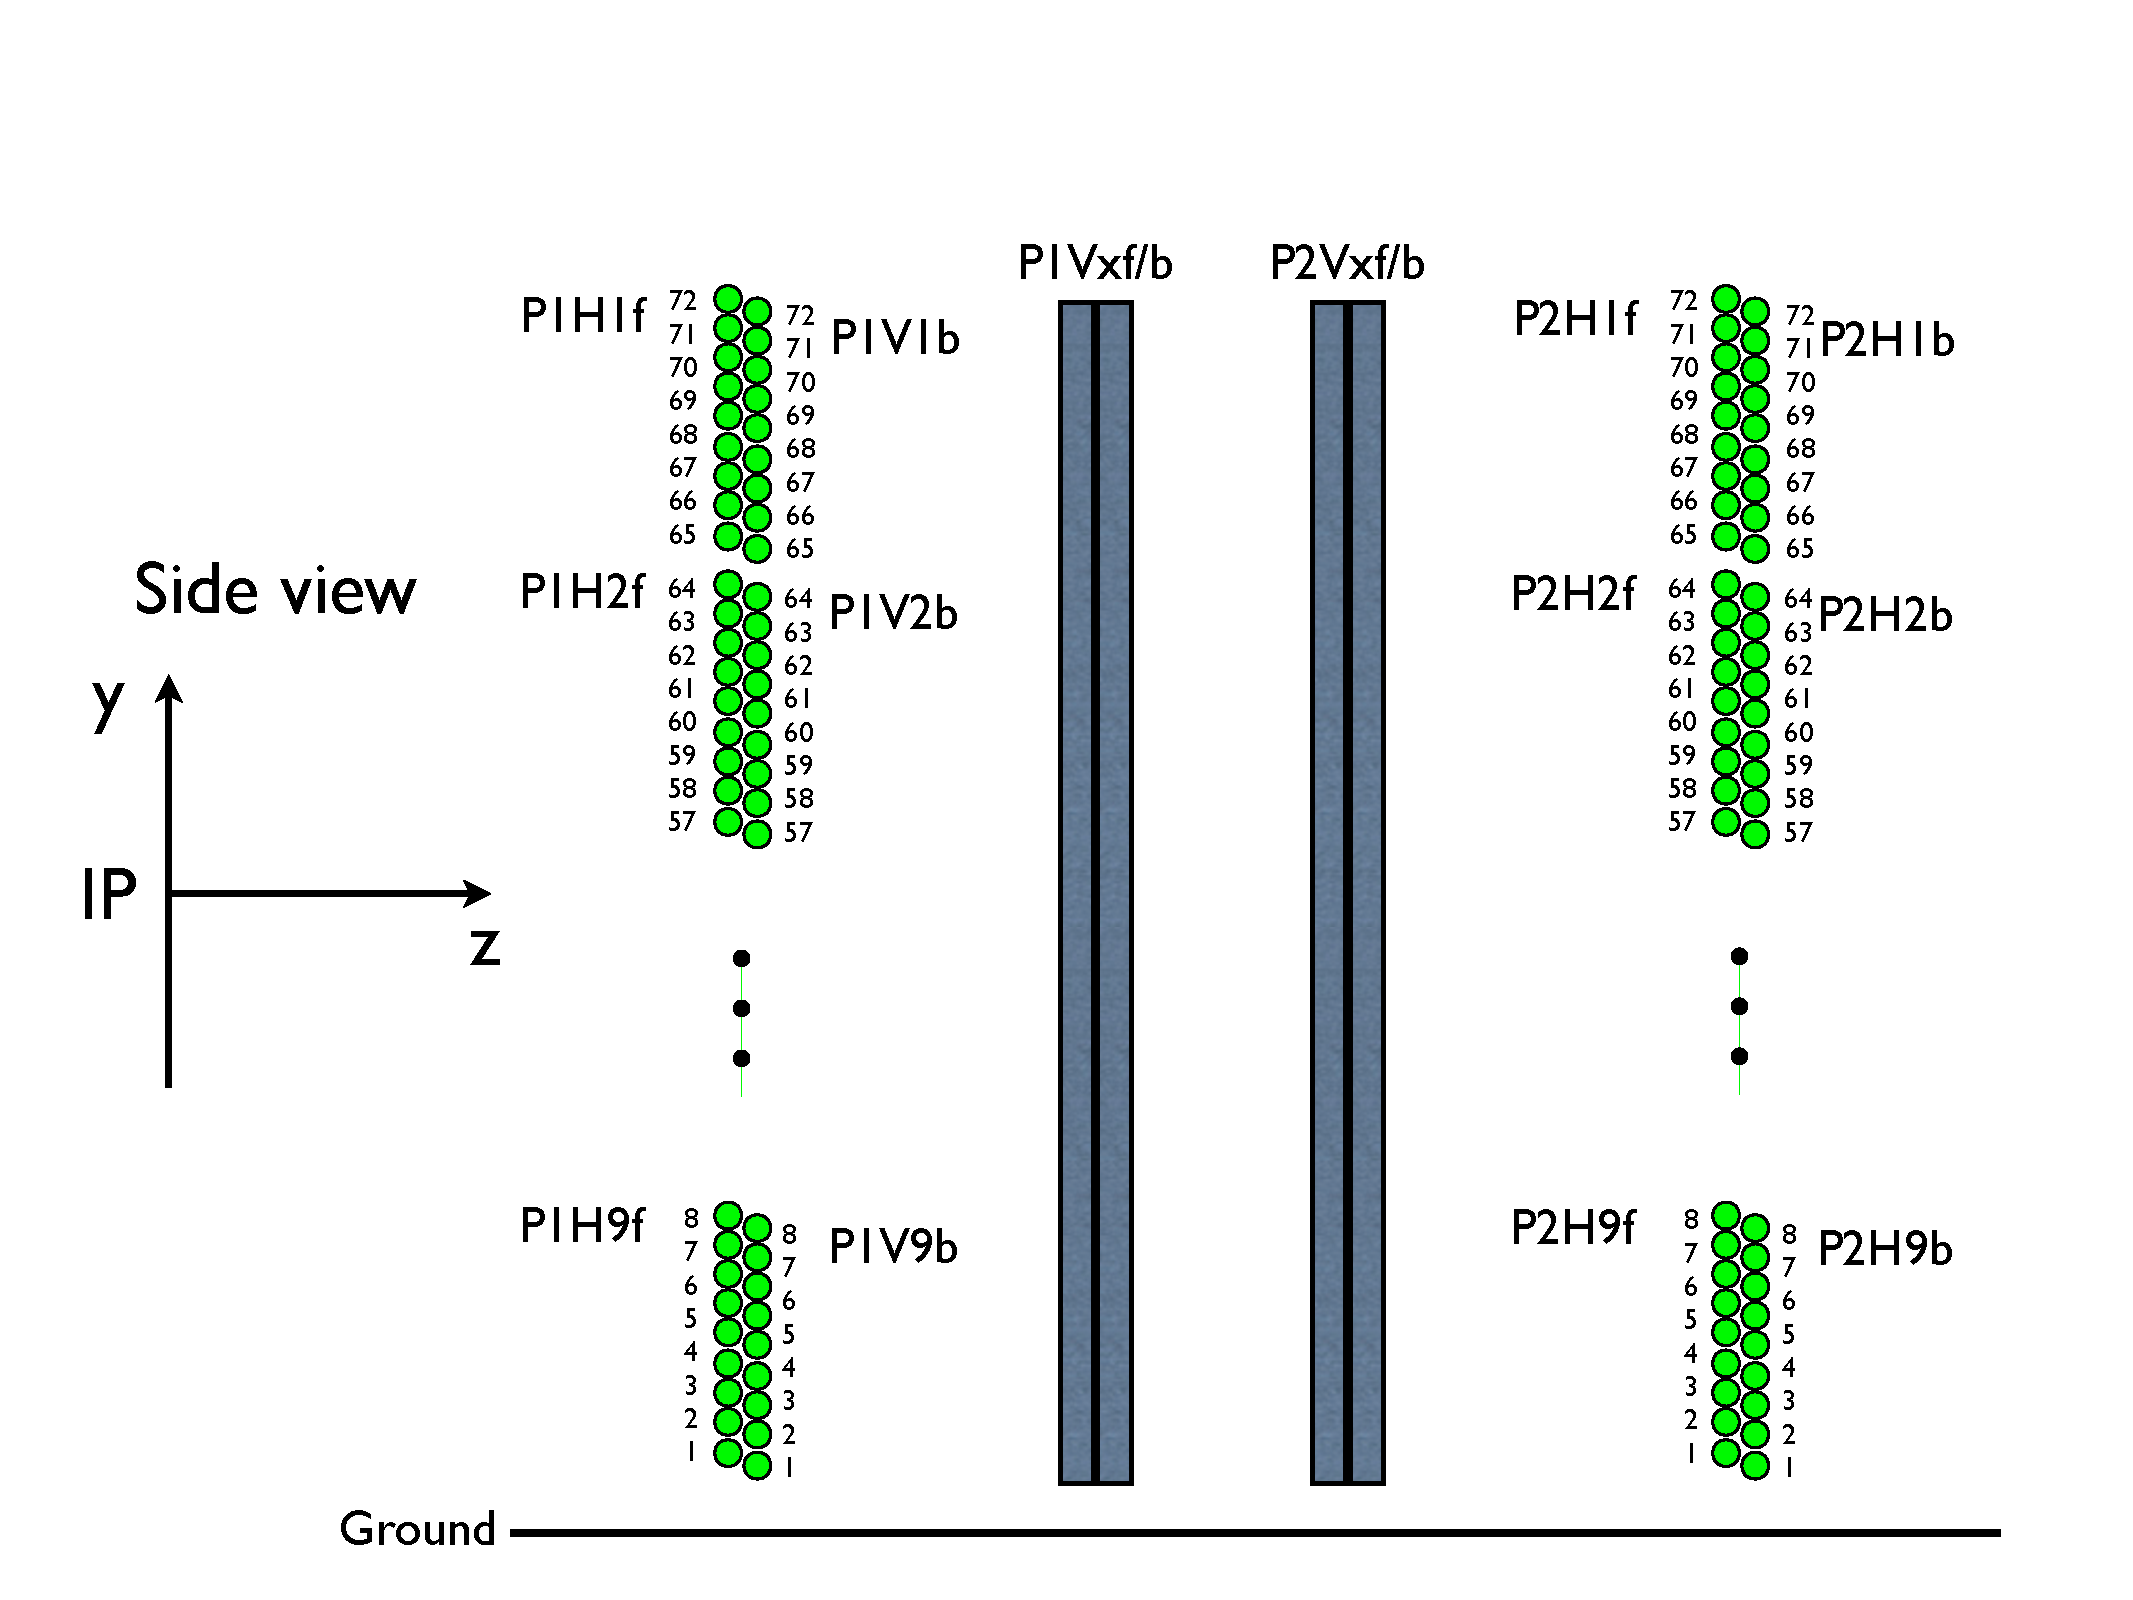
\includegraphics[width=1.03\linewidth]{figures/apparatus/proptubeview_yz.pdf}
		\caption{Proportional tube side ($y-z$ plane) view.}
		\label{fig:proptube:yzview}
	\end{minipage}
\end{figure}

Each plane of proportional tubes is composed of 9 \emph{modules}, each having a set of 16 proportional tubes: 8 in line in a horizontal or vertical orientation and 8 more offset (``primed'') from the first 8 by 0.5 inches. This offset structure prevents any muons from going undetected between tubes and allows for left-right disambiguation for two hits in adjacent primed-unprimed sub-plane pairs in the same module. The modules are labeled $1-9$ in increasing order from left to right for the $x-$measuring planes and from $1-9$ in increasing order from top to bottom. So, the top module of the first vertical plane of prop tubes is P2H1. Additionally, in each module, the primed and unprimed sub-planes are referred to as \emph{f} for ``front'' (facing upstream) and \emph{b} for ``back'' (facing downstream). This substructure can be seen in detail on Fig.~\ref{fig:proptube:xzview} and Fig.~\ref{fig:proptube:yzview}.

A single prop tube is made of 2-inch diameter aluminum tubes with a wall thickness of 1/16 inches. The central anode wire is a gold-plated $20 \mu$m diameter tungsten wire kept at approximately 1.95 kV. Considering the staggered nature of each plane's substructure, one can in principle achieve a spatial resolution of 0.3mm.  During Runs 2 and 3 of data taking, a resolution of 0.5mm for high energy muons was observed, which is more than sufficient for muon identification purpose. The gas mixture for prop-tubes is P-10 (Ar:Methane = 90:10) mixed with a $10\%$ CF4 gas (Ar:CO$_2$:CF$_4$ = 70:20:10) which yields the maximum drift time about 400ns. With this maximum, the prop tubes can handle a singles rate up to 2MHz while normal operational hit rates are typically below 1MHz.

A typical desired high-energy muon within spectrometer acceptance will traverse through two prop-tubes in each plane and induces hit signals on two anode wires. The path of a track is reconstructed from the drift time measured on the two anode output, with a custom TDC board that provides 0.44 ns timing resolution. With the hit information reconstructed from readouts of the forward and backward planes in $x-z$ and $y-z$ direction, precise reconstruction of the track trajectories can be obtained. Ideally, 8 hits from the 4 planes are used to form a track pointing back to the target. If such is the case, a candidate muon track is successfully identified.

\begin{table}[bthp]\centering
	\begin{tabular}{c|ccccc}
		\hline \hline
		Detector & Number       & \# tubes     & Width ($x$)               & $z$-position \\
		Plane     & of modules    & per         & $\times$ height ($y$)      & of front (back)   \\ 
		&                & module      & [cm] $\times$ [cm]        & sub-plane    [cm]    \\ 
		\hline
		P1H    &  9     & 16  & 368 $\times$ 368 &  2,099 (+4)    \\
		P1V    &  9     & 16  & 368 $\times$ 368 &  2,175 (+4)    \\
		P2V    &  9     & 16  & 368 $\times$ 368 &  2,367 (+4)    \\
		P2H    &  9        & 16  & 368 $\times$ 368 &  2,389 (+4)    \\
		\hline
		\hline
	\end{tabular}
	\caption{Parameters of the four proportional tube planes.}
	\label{table:prop:param}
\end{table}

\subsection{Mass Resolution from Chamber Resolution}

The mass resolution of the spectrometer is, in part, limited by the resolution of the tracking chambers and the distances between them. For an arbitrary set of hit positions in Stations 1, 2, and 3 ($r_1, r_2, r_3$) which are separated from each other in $z$ by distances $z_{12}$ and $z_{23}$, with KMAG in between Stations 1 and 2 supplying a $P_{kick}$, one can derive $\Delta P / P$. A line, or track segment, is first reconstructed between $r_2$ and $r_3$. The slope (and its uncertainty) of this track segment in the $z-x$ plane is:
\begin{equation}
s_{23} = \frac{r_3 - r_2}{z_{23}} \ \ ,\ \ \Delta s_{23} = \frac{1}{z_{23}}\sqrt{\Delta r_3^2 + \Delta r_2^2}
\end{equation}
The values of $\Delta r_n$ here are the position resolutions of the individual tracking chambers at each Station. One can use this slope to project a trajectory through KMAG and onto Station 1. The momentum is calculated by seeing where the actual hit position is in Station 1 and looking to the distance ($d$) between where the particle hit the station and where it would have hit had KMAG's magnetic field not existed. This is called a \emph{sagitta analysis}, as the magnetic field moves the particle's trajectory as if along a circle, and we are looking to the particle's path along the sagitta of that circle. Ultimately, the momentum uncertainty is related to this distance as:
\begin{equation}
\frac{\Delta P }{P} = \frac{P}{P_{kick}}\Delta d
\end{equation}
The expected sagitta point ($r_s$) is located at:
\begin{eqnarray}
r_s & = & s_{23} z_{12} + r_2 \\
\Delta r_s = \sqrt{\Delta s_{23}^2 z_{12}^2 + \Delta r_2^2} & = & \sqrt{ \Delta r_3^2 \left(\frac{z_{12}}{z_{23}}\right)^2 + (1+\left(\frac{z_{12}}{z_{23}}\right)^2) \Delta r_2^2}
\end{eqnarray}
\begin{figure}[t]
	\centering
	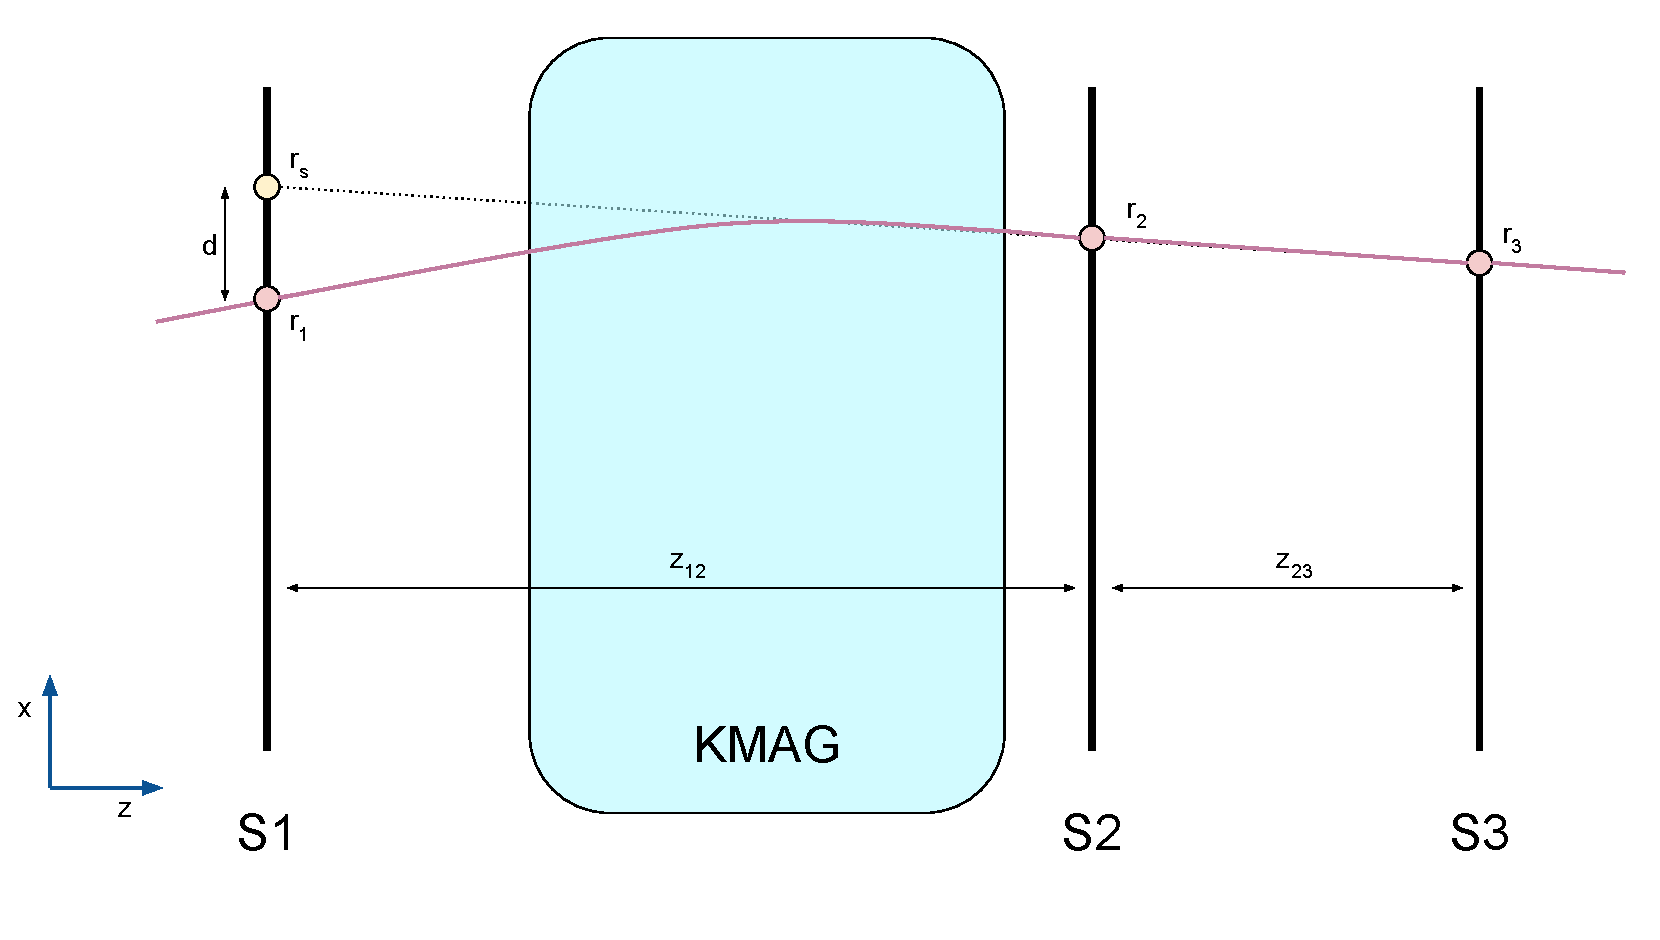
\includegraphics[width=0.75\textwidth]{figures/apparatus/momentum-resolution.pdf}
	\caption{A simplistic depiction of a track passing through from Station 1, through KMAG where its path is bent by the magnetic field, and then straight on through Stations 2 and 3.}
	\label{fig:mom-res}
\end{figure}
And the distance, $d$ follows as:
\begin{eqnarray}
d & = & r_s - r_1 \\
\Delta d = \sqrt{\Delta r_s^2 + \Delta r_1^2} & = & \sqrt{ \Delta r_3^2 \left(\frac{z_{12}}{z_{23}}\right)^2 + (1 + \left( \frac{z_{12}}{z_{23}} \right)^2) \Delta r_2^2 + \Delta r_1^2}
\end{eqnarray}
The momentum resolution due to chamber resolution can therefore be described as:
\begin{equation}
\frac{\Delta P}{P} = \frac{P}{P_{kick}} \sqrt{ \Delta r_3^2 \left(\frac{z_{12}}{z_{23}}\right)^2 + \left(1 + \left( \frac{z_{12}}{z_{23}} \right)^2 \right) \Delta r_2^2 + \Delta r_1^2}
\end{equation}
The dependence of the resolution on $P/P_{kick}$ works such that the larger the $P_{kick}$ is (w.r.t. particle momentum $P$), the more the track is bent, and the more precisely the original momentum is defined. Besides chamber resolution, other contributions to this momentum resolution are from multiple scattering through FMAG's iron beam dump and from the spectrometer's angular resolution. These will be discussed elsewhere in this paper.

The mass resolution is linked to momentum resolution via the following relation
\begin{equation}
\frac{\Delta M}{M} = \frac{\Delta P}{2 P}
\end{equation}
The factor of two arises from the fact that the Drell-Yan dilepton mass comes from two independent muons with the same momentum resolution. This mass resolution is important because it, in turn, contributes to the $\Delta x_2 / x_2$ resolution, which is the key dependent variable for SeaQuest measurements.
\begin{equation}
\frac{\Delta x_2}{x_2} \approx 0.57 \Delta x_F + 0.012 M^2 \frac{\Delta M}{M}
\end{equation}

\section{Trigger}

The SeaQuest Trigger System is designed to quickly select candidate dimuon events from the high-rate, high-background environment using discriminated hodoscope signals.

\subsection{Design Requirements}

%% DY selection, trigger rate
The trigger must select events of interest to the main physics goals with good enough efficiency (maximum signal-to-background ratio) to facilitate high-statistics analyses. In general, it is optimized to accept high-mass ($4-10$GeV) dimuons originating from the targets and beam dump. The event selection is also designed to intentionally reduce acceptance of dimuons from other, higher-rate sources, such as $J/\Psi$ decays and non-Drell-Yan dimuons originating from the beam-dump, though enough $J/\Psi$ events are triggered on to allow high-statistics analysis of $J/\Psi$ physics. Other goals of the trigger design are to keep the triggering rate low enough to maintain an acceptable DAQ livetime and to keep the trigger's internal throughput deadtime-free. By design, there should be no bottleneck at this stage, and the trigger should be capable of firing on any and all RF-buckets while the DAQ is live.

%% Flexibility
The hardware, firmware, and design should be sufficiently flexible to quickly accommodate changes in the spectrometer, beam conditions, and physics goals. Any changes to the geometric acceptance of the spectrometer, such as new/moved detectors or changes in the magnetic fields must be immediately reflected in the trigger selection in order to maintain high signal efficiency and good background rejection power. Similarly, a change in the beam duty factor or intensity should be accompanied by a change in the event selection, ensuring trigger rate optimization and zero internal deadtime. Finally, the trigger should be capable of specific modifications to facilitate special runs for other physics goals. For these reasons, the design of the trigger system underscores a significant need for flexibility in its hardware and design.

\begin{figure}[t]
	\centering
	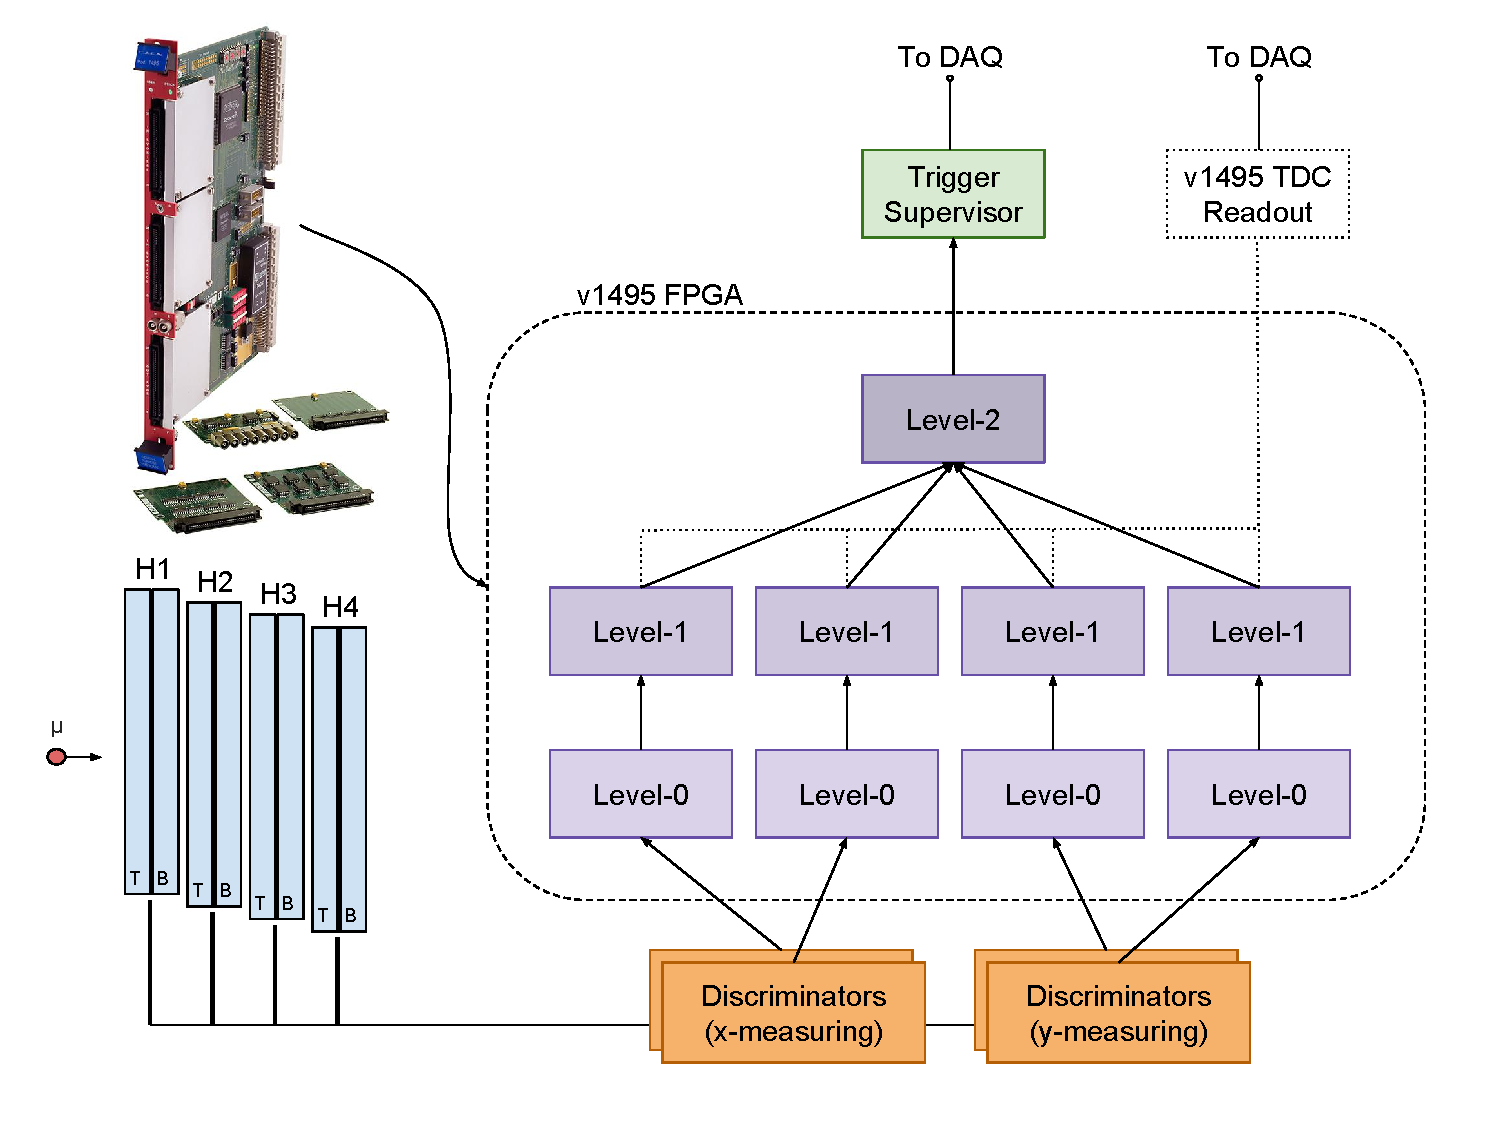
\includegraphics[width=0.75\textwidth]{figures/apparatus/v1495-trigger.pdf}
	\caption{The trigger system at SeaQuest is composed of 9 CAEN v1495 FPGA modules. These modules output a trigger signal to the Trigger Supervisor, which tells the DAQ when to record data.}
	\label{fig:1495-trigger}
\end{figure}

%% Self-monitoring, transparent
Lastly, the design of the trigger system should include self-diagnostic capabilities, allowing for constant monitoring of the trigger system's performance. Internal pulser-testing is employed to test the function of each compiled firmware every time the trigger logic changes. For added transparency, data from the internal TDC's is used by online and offline software to monitor the self-consistency of the trigger for each recorded physics event.

\subsection{Trigger Hardware}

The triggering system, which is depicted in Fig.~\ref{fig:1495-trigger}, begins with the Stations 1-4 hodoscope arrays. Hodoscopes are used for this task as the time resolution and high speed is limited only by the speed of light through the scintillator paddles and secondary emission of electrons (through the stages of the PMTs. This occurs over the span of nanoseconds, which allows for fast triggering on RF buckets that occur every 19ns during spills. The hodoscope planes - both x- and y-measuring planes - are separated into top and bottom sections as far as triggering is concerned. The signals from the hodoscope arrays are passed through a set of discriminator modules, which will only pass a signal on to the rest of the trigger if there is enough of a signal from the PMT's past a preset threshold.

The output of the discriminators is passed along to one of the nine CAEN v1495 FPGA (Field Programmable Gate Arrays) VMEbus (Versa Module Europa) modules~\cite{caen:v1495}. This hardware trigger consists of a single decision stage with a three-step parallel pipeline. These steps are referred to as the \emph{level-0}, \emph{level-1}, and \emph{level-2} stage triggers. The detailed internal flowchart of the CAEN v1495 electronics can be seen in Fig.~\ref{fig:v1495-internal}.

\begin{figure}
	\centering
	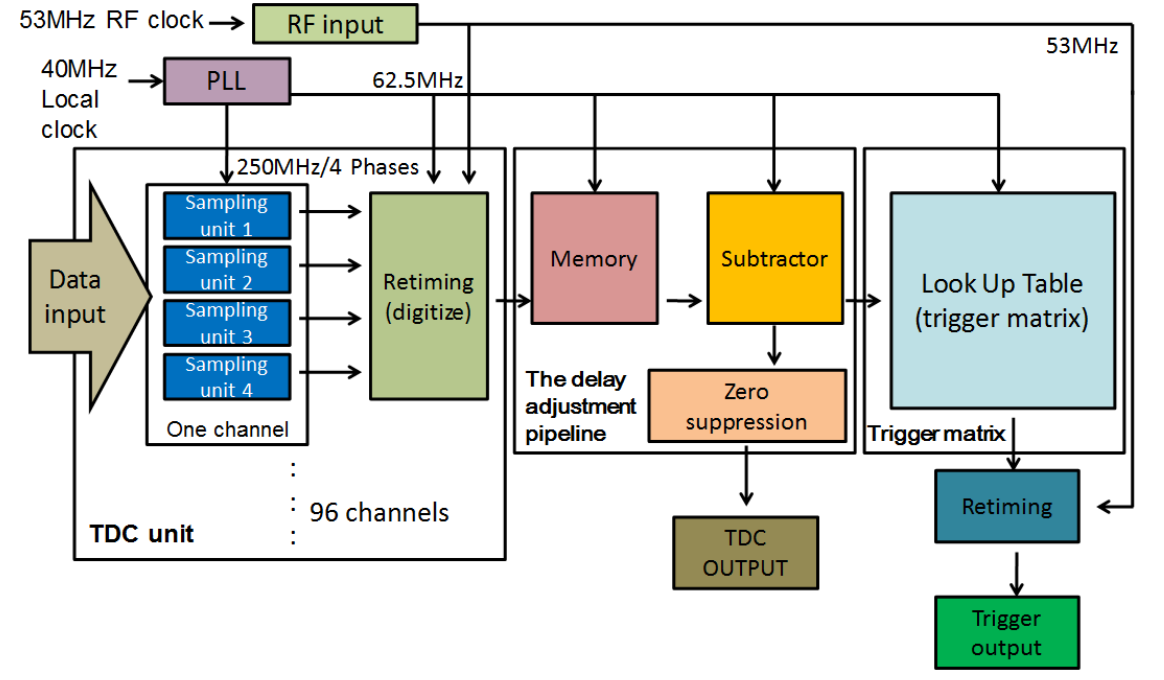
\includegraphics[width=0.75\textwidth]{figures/apparatus/trigger-block-diagram.png}
	\caption{A block diagram of the major functions of the v1495 FPGA~\cite{Shiu:2015ura}.}
	\label{fig:v1495-internal}
\end{figure}

At the first step, level-0, there is nothing actively performed during nominal data taking. The signal is passed on through, unaltered, to level-1. As it stands, level-0 is not used for any of the triggering modes. This stage is, however, extensively used for the pulser testing and self-diagnostic purposes. The level-0 stage is capable of being programmed to pulse arbitrary patterns on to the level-1 stage, which is very useful for observing how level-1 (and subsequently, level-2) will behave in a controlled setting. Whenever a new firmware is installed on the v1495, a pulser test is performed to ensure that all design requirements are met before uploading the firmware for production data taking.

The next level-1 trigger records the hit signals from the x- and y-measuring hodoscope hits split into top and bottom partitions with respect to their location in the SeaQuest spectrometer. The hit patterns are tested via a lookup table against a preselected set of hodoscope hit patterns, or \emph{``trigger roads''}. Each trigger road corresponds to a set of four hodoscopes: one from each station, with all being in the top or bottom half of the spectrometer. In this lookup table, there is a charge and approximate $p_T$ value for each preselected road. These are known via studies of Monte Carlo studies of muon paths from di- or single-muon events originating from the targets or beam dump. The roads were selected such that as many good dimuons are selected while reducing roads that are dominated by background signal that might cause trigger and/or DAQ deadtime.

During data taking, only the x-measuring hodoscopes were used for the v1495 trigger. As such, the two level-1 stages that look to the y-measuring hodoscope signals were unused. The level-1 trigger logic identifies four-out-of-four X1-X2-X3-X4 coincidences, which are characteristic of high $p_T$ single muons produced from the targets or beam dump. Each time a candidate coincidence that satisfies a preselected road is found, the level-1 step outputs certain logical bits indicating the track's charge, detector half (top or bottom), and $p_T$ bin.

The third step of the triggering logic is the level-2 trigger, or the \emph{``Track Correlator''} stage. This step takes the outputs of level-1 (charge, detector half, $p_T$ bin) and finds if any combinations satisfy any of the preprogrammed triggering modes. If one of these modes was satisfied, a signal is sent to the Trigger Supervisor (TS) module that communicates with the DAQ system to record an event at a specific synchronized RF bucket.

\subsection{Triggering Modes}

The v1495 FPGA had five configurable sets of physics triggers were used in the trigger system for the majority of production-level data taking. These five are referred to interchangeably as ``Matrix'' and ``FPGA'' triggers, followed by the number 1-5 indicating which of the five. These modes are described in detail in Table~\ref{tab:trigger-settings}.

\begin{table}[bthp]\centering
	\begin{tabular}{c|cccl}
		\hline
		Trigger & Condition       & Sign    & \#$\mu$ & Prescale\\
		\hline
		FPGA-1   & $T \land B$                        & Opposite  & 2        & 1    \\
		FPGA-2   & $(T \land T)\ \lor (B \land B)$  & Opposite  & 2        & 1000 \\
		FPGA-3   & $T \land B$                        & Same        & 2        & 123  \\
		FPGA-4   & $T \lor B$, all $p_T$            & $+ \lor -$& 1        & 30000\\
		FPGA-5   & $T \lor B$, $p_T > 3GeV$            & $+ \lor -$& 1        & 2000 \\
		NIM-1    & Y-coincidence                     & NA        & NA    & 30000\\
		NIM-2    & X-coincidence                    & NA        & NA    & 1000 \\
		NIM-3     & Random RF                        & NA        & NA    & 1000 \\
		\hline
	\end{tabular}
	\caption{Trigger settings for Run 3 and beyond. Prescale figures shown are typical values and were adjusted as experimental needs were tuned. NIM-1 and NIM-2 triggers' exact conditions could be changed and reconfigured from the counting room.}
	\label{tab:trigger-settings}
\end{table}

Different trigger settings were used for capturing data for different purposes. The primary triggering mode is FPGA-1, which looked for a combination of two roads of opposite sign that reside in opposite halves of the spectrometer. The FPGA-2 looked for good muon pairs that occurred in the same half. This, however, turned out to have a combinatoric problem that had two adverse effects: track reconstruction was difficult for these types of events, and the trigger fired off too often, causing high trigger and DAQ deadtime. As such, FPGA-2 was disabled for much of data taking. FPGA-3 trigger looked for the same kind of signal as FPGA-1, but with same-sign muon pairs. This type of event is useful for analyzing the experiment's combinatoric background. FPGA-4 and -5 are ``singles'' triggers that record events that are useful for estimating backgrounds and detector efficiencies. Each of these has a \emph{``prescale factor''} that limits how many of each mode actually fires the trigger. For example, FPGA-3 has a prescale factor of 123, which means that, within a single spill, there must be 123 FPGA-3 events before it tells the DAQ to record one. This keeps certain high-frequency trigger modes from dominating the readout and causing undue deadtimes.

In addition to the v1495 FPGA triggering mechanism, the outputs of the hodoscope discriminators are also sent up to the control room to a set of NIM logic modules. These signals, however, do not describe each hodoscope paddle but instead are \emph{AND}s of the tops and bottoms of each plane. For example, if one or more paddles in H1T fires, then a positive signal is sent out indicating that H1T fired. These signals can be used to form a rudimentary trigger on situations such as 4- or 3-out-of-4 coincidences in the X- or Y-direction hodoscope planes. In general, NIM-1 is used for Y-coincidences, and NIM-2 is used for X-coincidences.

The third NIM trigger mode is of particular importance, as it is used for estimating a great deal regarding backgrounds and rate dependence issues. The NIM-3 trigger is called the ``Random RF'' trigger, as it is controlled by two different clocks beating against each other. When the two clocks are in coincidence, they will send a signal to the Trigger Supervisor to record the event corresponding to the next immediate RF bucket. This trigger allows the experiment to get a random sample of the events that are occurring at the spectrometer, notably without a bias that a selective trigger can incur.

\section{Data Acquisition Systems}

The whole of the SeaQuest experiment spans two sectors of the NM beamline (NM3 and NM4) and records not only detector data but also accelerator and atmospheric conditions. Designing a data acquisition (DAQ) for this experiment, therefore, requires a bandwidth and timing which cannot be provided by a single central computer system. SeaQuest has therefore employed four separate DAQ subsystems called ``Main DAQ'', ``Scaler DAQ'', ``Beam DAQ'' and ``Slow Control''. The Main DAQ records the main detector information and the trigger timing. Scaler DAQ records various scaler readouts once per spill to reduce bias from the dead time of Main DAQ. Beam DAQ records information from a beamline \v{C}erenkov detector read out by its QIE board. The Slow Control is a catch-all for everything else, from magnet current to radiation monitors that are read out once per spill.

\subsection{Main DAQ}

The MainDAQ is powered by a Jefferson Lab developed software package named CODA (CEBAF\footnote{The old acronym inside of an acronym bit. CEBAF: Continuous Electron Beam Accelerator Facility} On-line Data Acquisition). The Trigger Supervisor could receive up to 12 different kinds of triggers. The first four triggers (FPGA 1-4) can be prescaled up to 24 bits. The second four triggers (FPGA 5, NIM 1-3) can be prescaled up to 16 bits. The rest of triggers (NIM4, flush trigger, Beginning of Spill (BOS), End of Spill (EOS)) are not prescalable. The Main DAQ can configure which triggers are enabled at the Trigger Supervisor level and what the  prescale factors are for each triggering mode. Once the TS receives a trigger, it will count the prescale factor and, based on how many triggers of that type have fired so far, it will decide if the Main DAQ will accept the trigger or not. 

Once the TS accepts the trigger, it sends an ``accepted trigger'' signal to the other front end electronics, such as the detectors' TDC readouts. Facilitating intercommunications, the Main DAQ system is connected to the TS and the CPU's in the VME crates via a local network. These CPU's are known colloquially at SeaQuest as readout controllers, or ``ROC's''. The TS connects with each VME crate, and when the TS sends an ``accepted trigger'', an interrupt signal is sent to each of the ROC's. The ROC's will then start reading the various front-end electronics (FEE).

The TS also sends a signal to the to QIE of the BIM, and the QIE retains information regarding the $\pm$16 RF buckets around that triggered RF bucket to assist in investigating the beam quality around each of our event triggers. The output of the QIE is encoded into a scaler latch card format. If the beam intensity in RF buckets neighboring the trigger is higher than the user-select threshold, then the board will issue a veto signal to the TS to ignore this trigger.

The Main DAQ's deadtime is considerable, as it has to communicate with the TDC's, which have the longest copy-in-progress time of \unit[32]{\us}. The average TDC readout time is approximately \unit[300]{ns} per 32bits (one hit), and as such, the slowest ROC which contains 7 TDCs has, on average, \unit[150]{\us} deadtime. This deadtime is accounted for under the umbrella term of \emph{``busy''} time and factored into the calculation of the ``live protons'' received by the experiment.

\subsection{Scaler DAQ}

The Scaler DAQ is used to ensure that the detector and trigger systems are working properly. The readout controller CPU is an MVME5500~\cite{mvme:scaler} with four scalers. One of these scalers is triggered by the coincidence of a \unit[7.5]{kHz} gate generator and the beam spill signal. This records the \unit[7.5]{kHz} response of the hodoscope arrays. The other three scalers are triggered by the BOS or EOS signals and thus record spill-level rates. Data collected by these spill-level scalers are the number of times each Main DAQ trigger is satisfied (both raw and accepted), the intensity of the beam, and the rates of the hodoscope arrays. The readout of this VMEbus DAQ is done using CODA very similarly to the Main DAQ but on a completely different system. An independent program analyzes the data in real-time in order to monitor the performance of the detectors and triggers, as well as the quality of the beam. 
%%An example of the ever-present online set of Scaler DAQ plots can be seen in Fig.~\ref{fig:scalerdaq}.


\subsection{Beam DAQ}

The Beam DAQ is composed of a \v{C}erenkov detector in the proton beam (the Beam Intensity Monitor discussed earlier in this chapter), a QIE board, and a custom C++ program to control their operation and read out. The Beam DAQ is responsible for recording the \unit[53]{MHz} structure of the beam, i.e. the intensity of each RF bucket. Its calculation of the \unit[53]{MHz} duty factor $DF=\frac{<I>^{2}}{<I^{2}>}$ is the primary measure of beam quality that accelerator operators use for tuning. In short, the duty factor is a measure of the \emph{uniformity} of the intensity of the beam. If we were to ignore the buckets intentionally left empty, and if it were to be the case that every RF bucket had the same number of protons, the \unit[53]{MHz} duty factor would be 100\%.

There four types of data recorded by the QIE have already been covered in the Beam Intensity Monitor section: QIESum, beam inhibit, busy time, and the $\pm16$ RF bucket intensities. The Beam DAQ commences read out of each of these blocks of data when the EOS signal is seen. The block of QIE data for all buckets is about \unit[300]{MB}. To read this much data in time to analyze it and be ready for the next spill, the DAQ program utilizes multithreaded processes. Three threads are used to read the data from the QIE board's three ethernet chips, and up to eight threads are used to analyze the data. Analyzed data is displayed on a public webpage so that shifters and accelerator operators can monitor the quality of the beam (Fig.~\ref{fig:beamdaq}). The fully processed data is also written out to tab-delimited ASCII files, which are archived and also uploaded to our online MySQL server.

\begin{figure}
	\centering
	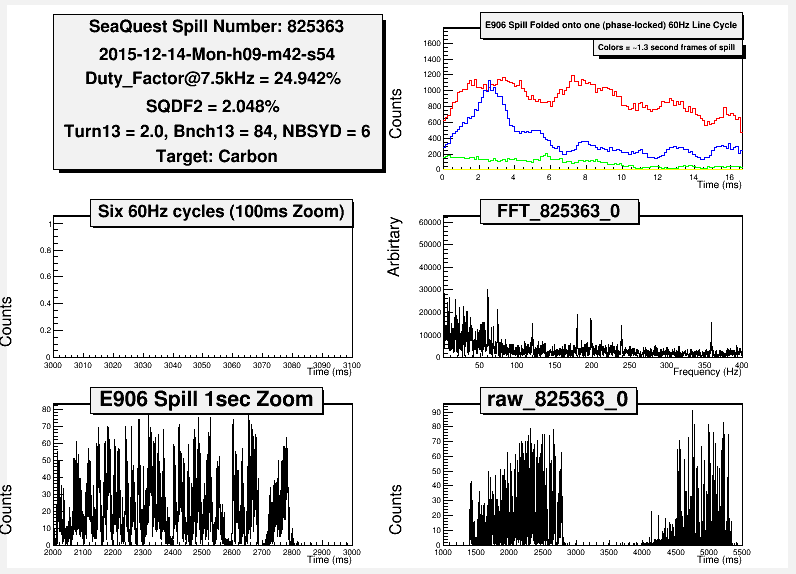
\includegraphics[width=0.75\textwidth]{figures/apparatus/E906FFT-scalerDAQ.png}
	\caption{A standard Beam DAQ display showing beam characteristics and spill data. The bottom two plots show the output of the QIE on a \unit[]{ms} scale.}
	\label{fig:beamdaq}
\end{figure}

\subsection{Slow Control Readout}

The Slow Control readout system is an aggregation of many different readouts from various parts of the experiment. This is also the umbrella term for other critical monitoring and bookkeeping tasks that must be performed. The one common thread to them all is that they only \emph{need} to be read out / performed once per spill in order to give perspective on the conditions of the experiment for each given spill. The term \emph{``Slow''} in Slow Control is adapted from the term ``Slow Spill'', which is used to characterize the method of beam delivery to SeaQuest. The Slow Control is run by an array of Python, Perl, and Bash scripts that, for the most part, run independently. These scripts primarily interact with and read out from EPICS, ACNET, and the local Spill Counter.

\subsubsection{EPICS, ACNET, and Kiethley}

The EPICS software package (Experimental Physics and Industrial Control System) is used for communicating any number of variables across the experiment's local network. EPICS is used for feeding readouts from many different sources and formats, and making them available to any other system that may have need of certain information, but does not natively communicate with a different system's format. Bridging this gap, EPICS is able to gather information regarding the target, beam, and environmental data into one place.

The EPICS server is installed on SeaQuest's target control computer, where the target position, pressures, temperatures, and proximity sensors are monitored and controlled. These values are critical to track and monitor, as they affect what target is in position at any given spill, along with information that may infer the cryogenic liquid targets' densities. Additionally, there is information regarding the operational mode of the target table, such as whether or not the target table is being manually controlled or if it is automatically repositioning itself. In Slow Control parlance, information from the target computer that is sent to the EPICS server is labeled as ``Target'' type data.

Several values are read into the EPICS server from the Accelerator Network (ACNET), which monitors many critical systems. Beam intensities (S:G2SEM) and FMAG / KMAG currents are two of the major factors that must be factored in for any analysis. There are additional readouts with esoteric names that can record anything from beam pipe vacuum to upstream radiation monitors. It is important to note that the FMAG and KMAG variables from ACNET are read out to the EPICS server every \unit[3]{s}, particularly because it is unsafe to deliver beam to the sensitive detectors without FMAG being fully powered. As such, the FMAG current is read into the beam interlock system. In the Slow Control feed, this type of information is labeled as ``Beam'' data.

Finally, there is a Keithley multimeter \CN in SeaQuest Hall near the electronics racks by Station 3. This device has the responsibility of relaying information regarding ambient temperature, air pressure, and humidity up to the control room. This information on its own is not typically used for any analyses, but in the case that, for example, a rise in humidity results in any electrical device failures, the monitoring data exists to diagnose it as such. This data is gathered by a `kscan' program that is run on the target machine, and its operation typically takes 11s to return a result. Data from the Keithley multimeter that is put into the Slow Control feed is labeled as ``Environment'' data.

\subsubsection{Spill Counter}

Perhaps one of the most critical components of the data acquisition is the coordination between the many sources of data in the DAQ. The Main DAQ, Scaler DAQ, Beam DAQ, and Slow Control do not share a single clock or network, so some measures need to be taken to ensure that data from different sources regarding a single spill's worth of data actually all correspond to the same spill. The concept of a locally maintained Spill Counter arose as a solution to this problem, and it is handled in the form of a simple Python script and a flat text file containing a single integer.

The enacted solution begins with placing an initialized spill counter (\emph{spillID})value (currently \emph{O}($10^5$)) into an otherwise empty text file at a specified location. Then, when the ACNET readout receives a BOS/EOS signal from AD, a simple python script performs the following:
\begin{itemize}
	\item Read the current spillID from the file
	\item Broadcast this value over the EPICS server
	\item Insert a single ASCII-encoded event into the Main DAQ and Scaler DAQ CODA streams containing only that spillID number
	\item Waits for \unit[20]{s} while other scripts may want to use the current spillID value to connect its value to the spill that just ended
	\item Updates the file to contain spillID + 1
\end{itemize}

This simple approach has been very effective in its usage so far, and the spillID incremented via this method has been shown to be accurate upon scrutiny of data contents across DAQs. This can be easily done by looking at a series of full and empty spills, as it is obvious which spills had a nominal beam spill and which did not by investigating the output of each DAQ. The weakness lies in the fact that this system relies on a single file, which is susceptible to any number of file access and timing issues. At some point in the future, it would be advisable to have all spillID-using systems to read the current value from the broadcasted EPICS server value instead of having several applications attempting to access and read the single file (even if just read-only).

\subsubsection{Python Slow Control Script}

With all of this going on to aggregate data from several sources, there is one final script that takes this aggregated data and makes it readily available for the rest of the DAQ systems. A \verb|read_slowcontrol.py| script, once every \unit[60]{s} supercycle, puts the following together into a single ASCII text file:
\begin{itemize}
	\item Clock time (``vxticks'') of the Trigger Supervisor
	\item Spill count data
	\item Beam data
	\item Environmental data
	\item Target data
	\item Timestamp
\end{itemize}

Once all of this is written to a file, this is sent to the Main DAQ and Scaler DAQ to be integrated into the full CODA file as a plain text event with a simple, tab-delimited format.